%%%%%%%%%%%%%%%%%%%%%%%%%%%%%%%%%%%%%%%%%%%%%%%%%%%%%%%%%%%%%%%%%%%%%%%%%%%%%%%%%%%%%%%%%%%%%%%%%%%%

\chapter{Star formation and star forming galaxies}
\chaptermark{star formation}
\label{introduction: chapter: star formation}

%%%%%%%%%%%%%%%%%%%%%%%%%%%%%%%%%%%%%%%%%%%%%%%%%%%%%%%%%%%%%%%%%%%%%%%%%%%%%%%%%%%%%%%%%%%%%%%%%%%%

\section{Star formation in molecular clouds}
\label{introduction: section: star formation: SF in clouds}

\subsection{A sketch of the star formation process}
\label{introduction: section: star formation: sketch}

If the gravitational force of a molecular clouds mass overcomes potential stabilizing forces, the cloud will collapse to smaller size and higher density. In this process, the clouds usually fragments into cores that can collapse faster than the overall cloud.
Eventually, the collapsing pre-stellar core stabilizes due to radiation pressure of the beginning nuclear fusion but continues to accrete mass from the surrounding, still collapsing, cloud.
In massive clouds, enough mass is present for the formation of dozens to millions of stars which can remain bound in a stellar cluster or even super star cluster (Section~\ref{introduction: section: star formation: SSCs}). 

A newly formed proto-star is still embedded in the cloud from which it formed and it is therefore challenging to observe this phase of star formation. Infrared radiation from the cloud core and proto-star can escape the cloud but, especially for massive and dense clouds, longer wavelengths in the sub-mm regime subject to less extinction are required.
After its birth, a (proto-)star begins to dissociate and disperse its natal cloud through proto-stellar outflows and radiation (feedback, Section~\ref{introduction: section: star formation: feedback}) with the help of its siblings formed in the same cloud. 
The diverging size scales in star formation from stars (R$_\odot \sim 10^{-8}$\,pc) in cloud cores ($\LESSSIM$ pc) embedded in GMCs (up to $200$\,pc) that are influenced by galactic processes (several kpc) make it difficult to understand and model these early phases.


\subsection{Why is star formation inefficient?}
\label{introduction: section: star formation: inefficiency}

Of course, star formation is much more complicated than the simple sketch outlined above and many details of the star formation process are known today. However, there are still fundamental problems yet to be solved and understood in detail.
In the following, one important complex of problems is highlighted since they are related to this thesis.

\begin{figure}[t]
	\centering
	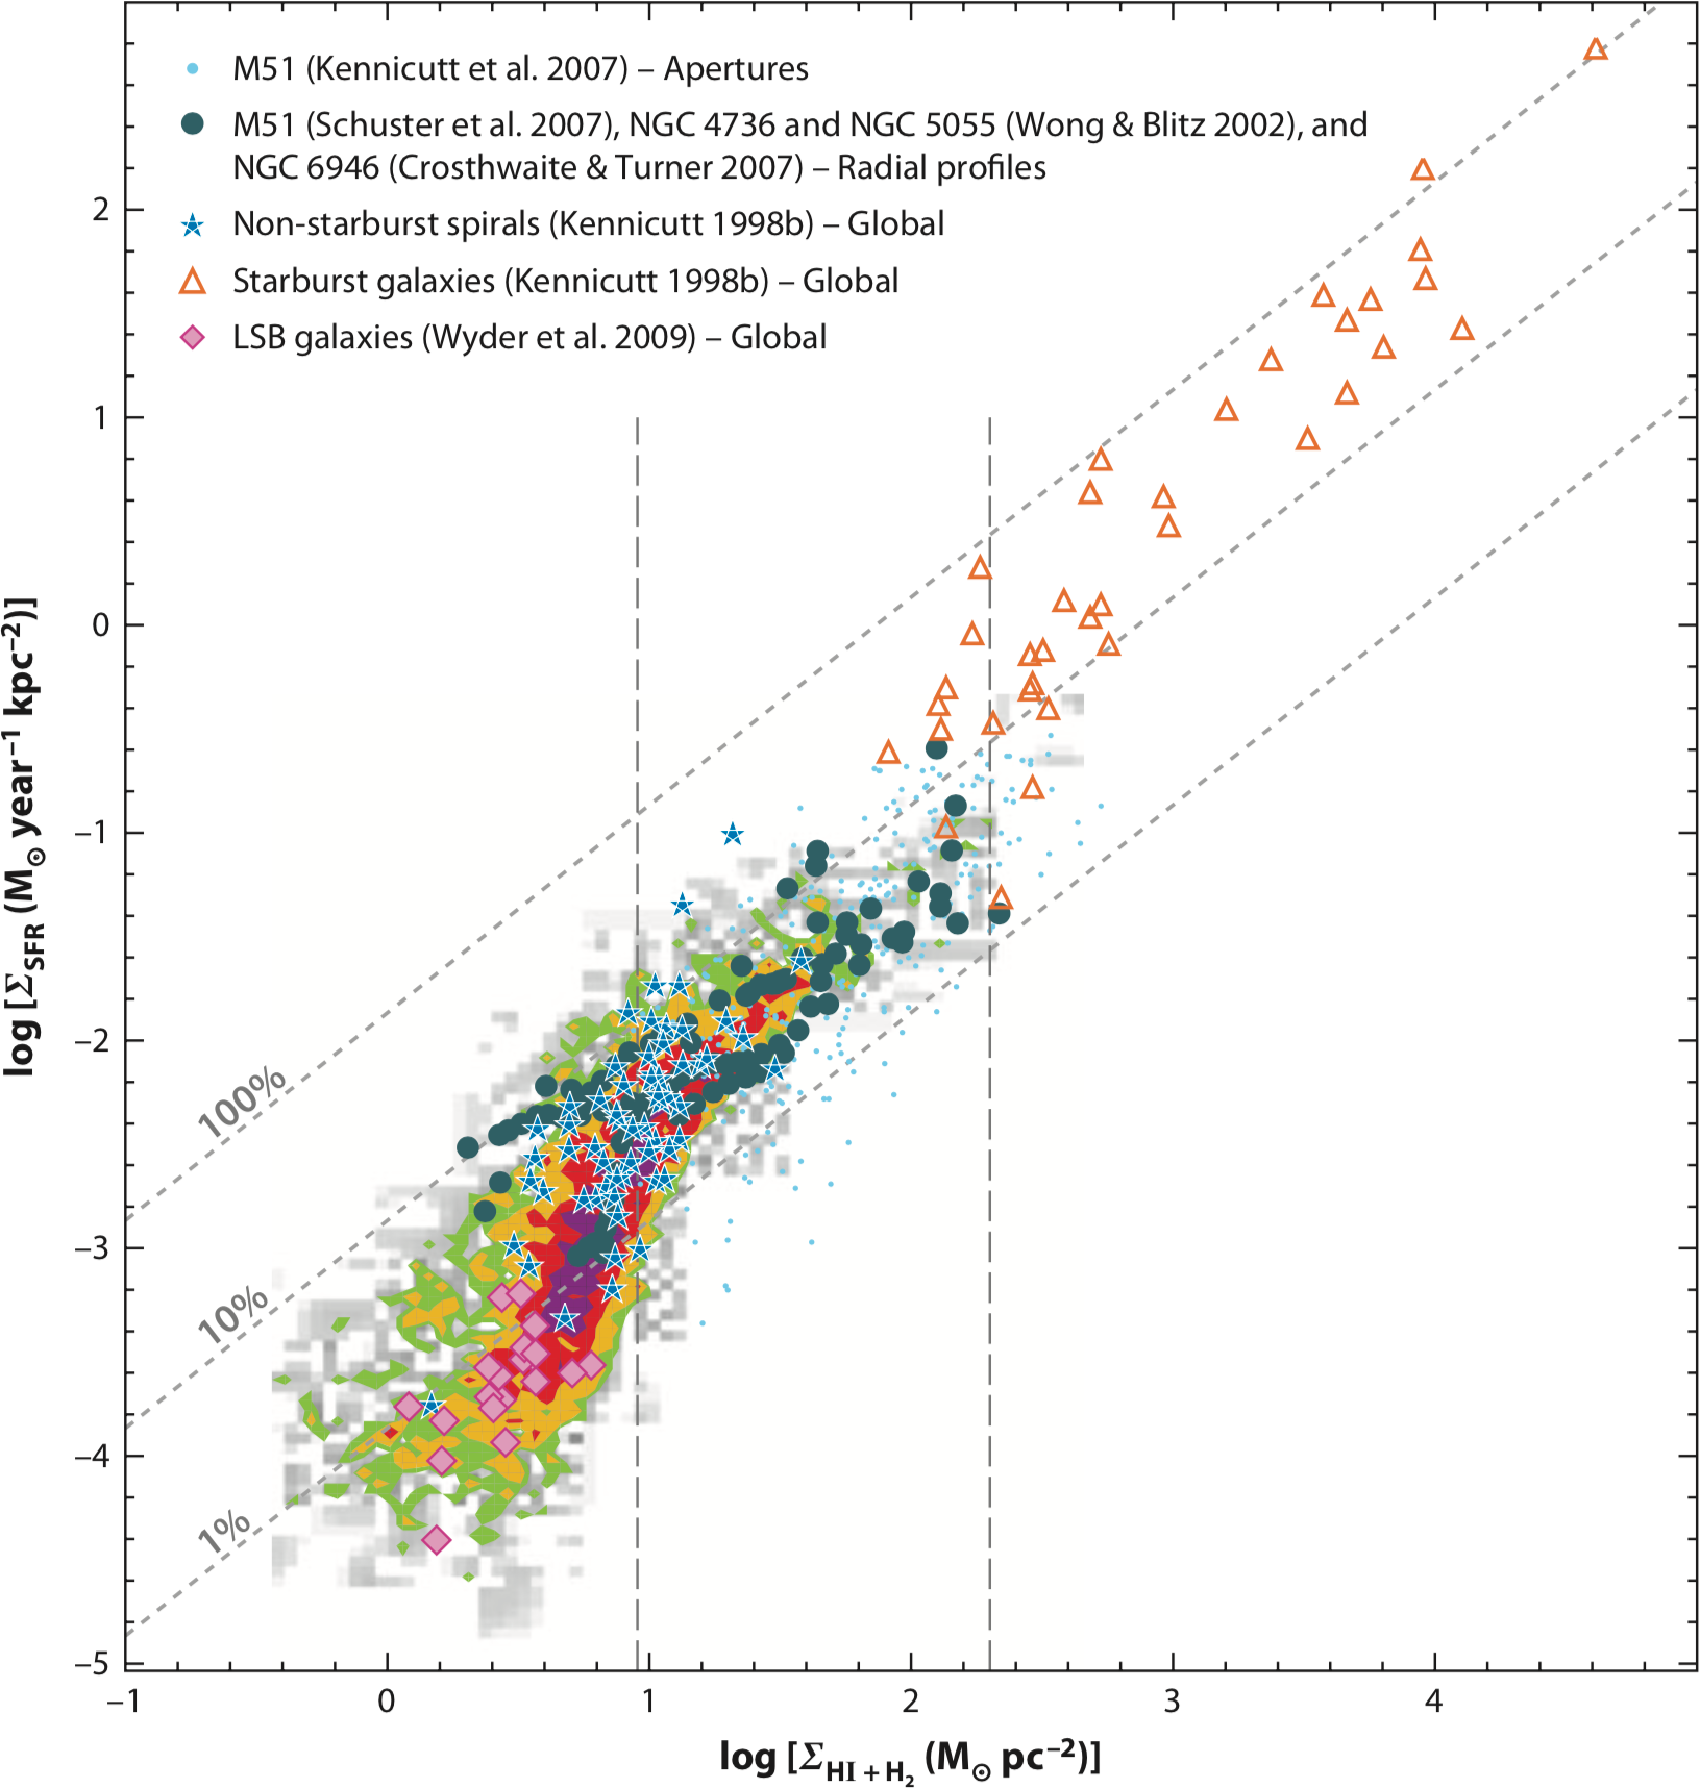
\includegraphics[width=0.8\linewidth]{images/chapters/introduction/sf/SF_law.pdf}
	\caption[Star formation (Kennicutt-Schmidt) law]{The star formation law (Kennicutt-Schmidt law) relates gas surface density to star formation rate surface density. In this figure from (\citealt{2012ARA&A..50..531K}; in original form in \citealt{2008AJ....136.2846B}) the total gas as the sum of neutral and molecular gas is shown. Typical star forming galaxies have low star formation efficiencies of up to a few percent depending on observational details (e.g. aperture size, location in the disk) while starbursts convert gas into stars much more efficiently.}
	\label{introduction: figure: star formation: SF law}
\end{figure}

Star formation seems extremely inefficient when comparing the amount of available gas to the ongoing star formation and the number of young stars \citep[e.g.][]{2007ARA&A..45..565M,2014PhR...539...49K}.
On the scale of galaxies or kpc sized regions within galaxies, the star formation law (Kennicut-Schmidt law) $\Sigma_{SFR} \propto \Sigma_{gas}^n$ quantifies the correlation between (molecular) gas and star formation \citep{1959ApJ...129..243S,Kennicutt:1998id}. It relates star formation rate surface density $\Sigma_{SFR}$ to molecular or total (molecular and neutral) gas mass surface density $\Sigma_{gas}$.
\citet{Kennicutt:1998id} found $n = 1.4 \pm 0.15$ for HI observations as the average over 100 nearby galaxies while \citet{1959ApJ...129..243S} originally suggested $n \sim2$. 
Figure~\ref{introduction: figure: star formation: SF law} shows a compilation of the literature for the total gas mass from \citet{2012ARA&A..50..531K}.

The ratio of gas mass available to star formation and the observed SFR (or equivalently the respective surface densities) defines the gas depletion time $\tau_\mathrm{dep} = M_\mathrm{mol}/SFR$. 
The inverse of the depletion time is the star formation efficiency $SFE = \tau_\mathrm{dep}^{-1}$ and describes how much and how fast gas is converted into stars.
The SF law is therefore tightly linked to the (in-)efficiency of star formation and suggests star formation efficiencies of $\sim 10^{-9}$\,Gyr$^{-1}$ (or $\tau_\mathrm{dep} \sim 1$\,Gyr) in typical star forming galaxies.

The (star forming) gas is characterized by the free-fall time $\tau_\mathrm{ff} = \sqrt{3\pi / 32 G \rho}$ that depends entirely on the gas density $\rho$ and describes the time required for the gas to collapse. Alternative formulations of the $SFE = SFR/M_\mathrm{mol}$ also consider this natural timescale (and/or other timescales) of molecular clouds.

The star formation efficiency $\epsilon_\mathrm{ff} = \tau_\mathrm{ff} / \tau_\mathrm{dep}$ eliminates the time dependence of the SFE \citep{2005ApJ...630..250K} and observations show a nearly universal efficiency of order 1\% \citep[e.g.][]{Krumholz:2012ja,2018ApJ...861L..18U,2017A&A...604A..74S}.

The solution to the efficiency problem is not yet entirely clear. Studies of star formation across various size scales show a scale dependence such that, although star formation is very inefficient on large scales, the smallest structures such as cloud cores can reach $30-70$\% \citep{2013ApJ...763...51F,2014prpl.conf...77P}. In the context of turbulence regulated star formation models, this shows how cores can collapse efficiently while stabilizing forces (primarily turbulence, but also magnetic fields) can prevent other regions within a cloud from forming stars \citep[e.g.][]{2019ApJ...883....2S}.

Stellar feedback (Section~\ref{introduction: section: star formation: feedback}) is known to play an important role in generating turbulence, but other dynamical effects (e.g. magneto-rotational instability, accretion driven) on galactic scales contribute to the generation of turbulence\citep[e.g.][]{2019ApJ...871...17U}.
However, it is not yet understood how stellar feedback couples to the star forming gas to drive turbulence. One manifestation of feedback are outflows which could not yet be studied in detail (meaning at high spatial resolution on pc scales), a problem that this thesis addresses.

Figure~\ref{introduction: figure: star formation: SF law} also shows that starburst galaxies (Section~\ref{introdution: section: star formation: starbursts}) achieve much higher SFE than typical star forming galaxies. The path to a unified model of star formation therefore must include the study of starbursts. It needs to be better understood how exactly starbursts differ from other galaxies in their gas and star forming properties. This thesis presents important steps towards that goal by studying a particular starburst at highest resolution.


%%%%%%%%%%%%%%%%%%%%%%%%%%%%%%%%%%%%%%%%%%%%%%%%%%%%%%%%%%%%%%%%%%%%%%%%%%%%%%%%%%%%%%%%%%%%%%%%%%%%

\section{Super star clusters}
\label{introduction: section: star formation: SSCs}

\begin{figure}[t]
	\centering
	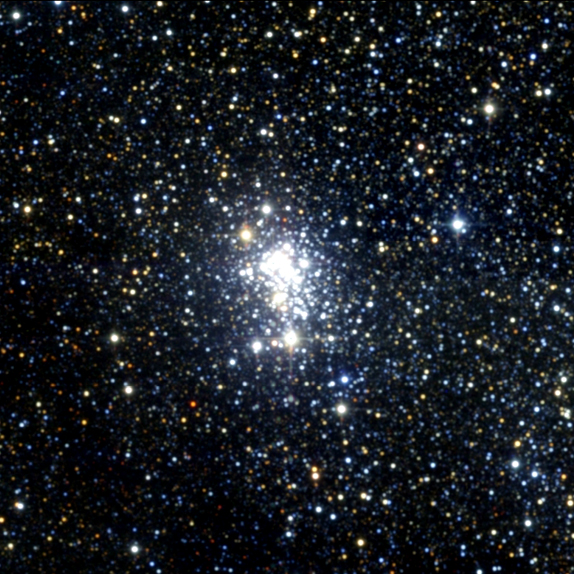
\includegraphics[width=0.6\linewidth]{images/chapters/introduction/sf/westerlund1_IR.jpg}
	\caption[Super star cluster Westerlund 1]{The super star cluster Westerlund~1 in the infrared as seen by the 2 Micron All-Sky Survey (2MASS). Westerlund~1 with a mass of $M_\ast \sim 6\times10^4$\,\Msun was the first SSC discovered in the Milky Way. Credit: 2MASS/UMass/IPAC-Caltech/NASA/NSF.}
	\label{introduction: figure: star formation: SSC example}
\end{figure}

For very massive molecular clouds, the product of the star formation process can be an also very massive stellar cluster, e.g. Arches \citep[$M_\ast = 10^{4.3}$\,\Msun;][]{1999ApJ...514..202F} and Quintuplet \citep[$M_\ast = 10^{4.0}$\,\Msun;][]{2006ApJ...643.1166F} in the Milky Way Galactic center or R136 in the Large Magellanic Cloud \citep[$M_\ast = 10^{4.78}$\,\Msun; e.g.][]{1995ApJ...448..179H,2009ApJ...707.1347A}.
Even more massive clusters can be found outside the local group and go by the name super star clusters (SSCs). The distinction from other stellar clusters is somewhat arbitrary and usually defined to cover the most massive ($M \GTR 10^5$\,\Msun) and very compact ($R \sim 1$\,pc) systems. SSCs are especially prevalent in starbursts like M82 or the antennae \citep[e.g.][]{2005ApJ...621..278M,2003dhst.symp..153W,2015ApJ...806...35J}.

SSCs are thought to be younger cousins of globular clusters \citep[e.g.][]{2015IJMPD..2430002B} and might thus help to understand the formation of old stellar systems and the evolution of galaxies (also see Section~\ref{introduction: section: star formation: cosmological context}). Globular clusters are massive ($M \GTR 10^5$\,\Msun), compact ($R \sim 10$\,pc) and very old ($\GTR 10$\,Gyr). Taking evolutionary effects (late-phase stellar mass loss, stars evaporating off the cluster, tidal interactions) into account, globular clusters must have formed with very high masses $M \GTRSIM 10^6$\,\Msun, similar to the most massive SSCs in the local universe.

To date, SSCs have been found in $\GTR20$ nearby galaxies including \ngc253 \citep{Watson:1996dn,Kornei:2009ee}, ESO338 \citep{2007A&A...461..471O}, \ngc5253 \citep{2017ApJ...846...73T}, M51 and M82 (see the review by \citealt{2010ARA&A..48..431P} for an overview).
Very young and still forming SSCs have been found in the Antennae \citep{2012A&A...538L...9H,2015ApJ...806...35J}, the Large Magellanic Cloud \citep{2017NatAs...1..784O}, \ngc253 \citep{2018ApJ...869..126L} and \ngc5253 \citep{2017ApJ...846...73T}. The high extinction of the large amounts of dense gas obscures potential young clusters and only recently it became possible to resolve SSC scales with ALMA in the less affected sub-mm wavelengths.
Chapter~\ref{chapter: SSCs} presents a study of the physical and chemical properties of the ISM in and around young (proto-)SSCs in \ngc253 with resolved observations for the first time.


%%%%%%%%%%%%%%%%%%%%%%%%%%%%%%%%%%%%%%%%%%%%%%%%%%%%%%%%%%%%%%%%%%%%%%%%%%%%%%%%%%%%%%%%%%%%%%%%%%%%

\section{The main sequence of star forming galaxies}
\label{introduction: section: star formation: main sequence}

Galaxies can be empirically grouped into different classes according to their location in the plane of star formation rate versus stellar mass (Figure~\ref{introduction: figure: star formation: MS}).
Galaxies of typically blue color are found to lie on a diagonal sequence, i.e. their star formation rate scales with stellar mass \citep[e.g.][]{2004MNRAS.351.1151B,2011A&A...533A.119E}. This relation is called the main sequence (MS) of star forming galaxies (SFGs).
Most other galaxies are located in a clumpy structure at low star formation rates nearly independent of stellar mass. Since these galaxies are passive and typically red in color, they are called red clump galaxies, or ``red and dead'' in colloquial terms.
Galaxies in the transition region are far more sparse and thus denoted green valley galaxies because they lie in between the peaks of red and blue galaxies.

\begin{figure}[t]
	\centering
	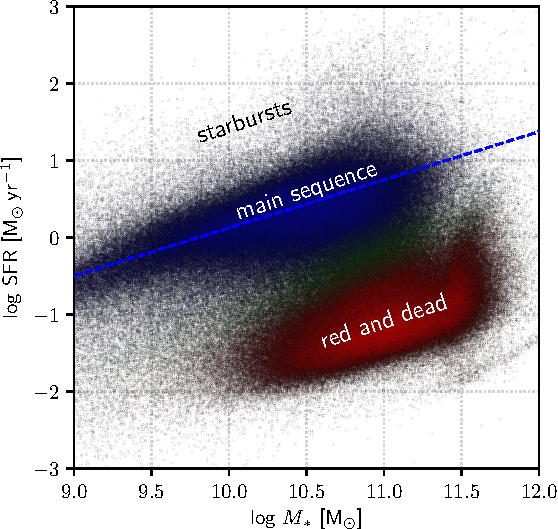
\includegraphics[width=0.6\linewidth]{images/chapters/introduction/sf/SDSS_main_sequence.pdf}
	\caption[Main sequence of star forming galaxies]{About 270,000 galaxies from SDSS DR8 sample the parameter space in the stellar mass vs. star formation rate plane and reveal a galaxy bimodality. The main sequence of star forming galaxies is an empirical relation on which typical starforming galaxies fall. Galaxies above the relation are called starbursts. Old, red, typically elliptical galaxies fall below the main sequence and after often referred to as ``red and dead''. The green valley is a name given to the transition region between starforming main sequence and quiescent red and dead galaxies.}
	\label{introduction: figure: star formation: MS}
\end{figure}

A single galaxy is not static in the stellar mass -- star formation rate diagram but can evolve through the different phases \citep[e.g.][]{2006MNRAS.368....2D,2018MNRAS.474.2039E}. Mergers or gas infall can trigger star formation and push the galaxy up into the starburst regime. When the gas is eventually consumed by star formation or has become unavailable to star formation by other processes, the galaxy moves down the diagram through the green valley to become a passive galaxy.

The position in the stellar mass -- star formation rate diagram correlates with galaxy morphology \citep[e.g.][]{2004MNRAS.351.1151B}. Red clump galaxies are typically elliptical (early Hubble types) while main sequence and starbursts are typically spirals (late Hubble types). Starburst galaxies are also often irregular in shape.


%%%%%%%%%%%%%%%%%%%%%%%%%%%%%%%%%%%%%%%%%%%%%%%%%%%%%%%%%%%%%%%%%%%%%%%%%%%%%%%%%%%%%%%%%%%%%%%%%%%%

\section{Starbursts}
\label{introdution: section: star formation: starbursts}

Starbursts are located above the MS at increased star formation rates. The distinction between MS and starbursts is based on the depletion time (Section~\ref{introduction: section: star formation: inefficiency}) of the molecular gas reservoir under the observed star formation rate. As mentioned before, normal star forming galaxies have typical depletion times $\tau_\mathrm{dep} \sim 1-2$\,Gyr \citep[e.g.][]{Leroy:2008jk} whereas starbursts consume their molecular gas at a much higher rate in $\tau_\mathrm{dep} \sim 0.1$\,Gyr \citep[e.g.][]{Kennicutt:1998id,2008AJ....136.2846B}.
The transition from MS to starburst is fluent and not coupled to a specific depletion time. Instead, the strength of a starburst can be parametrized as the offset from the MS.

\begin{figure}
	\centering
	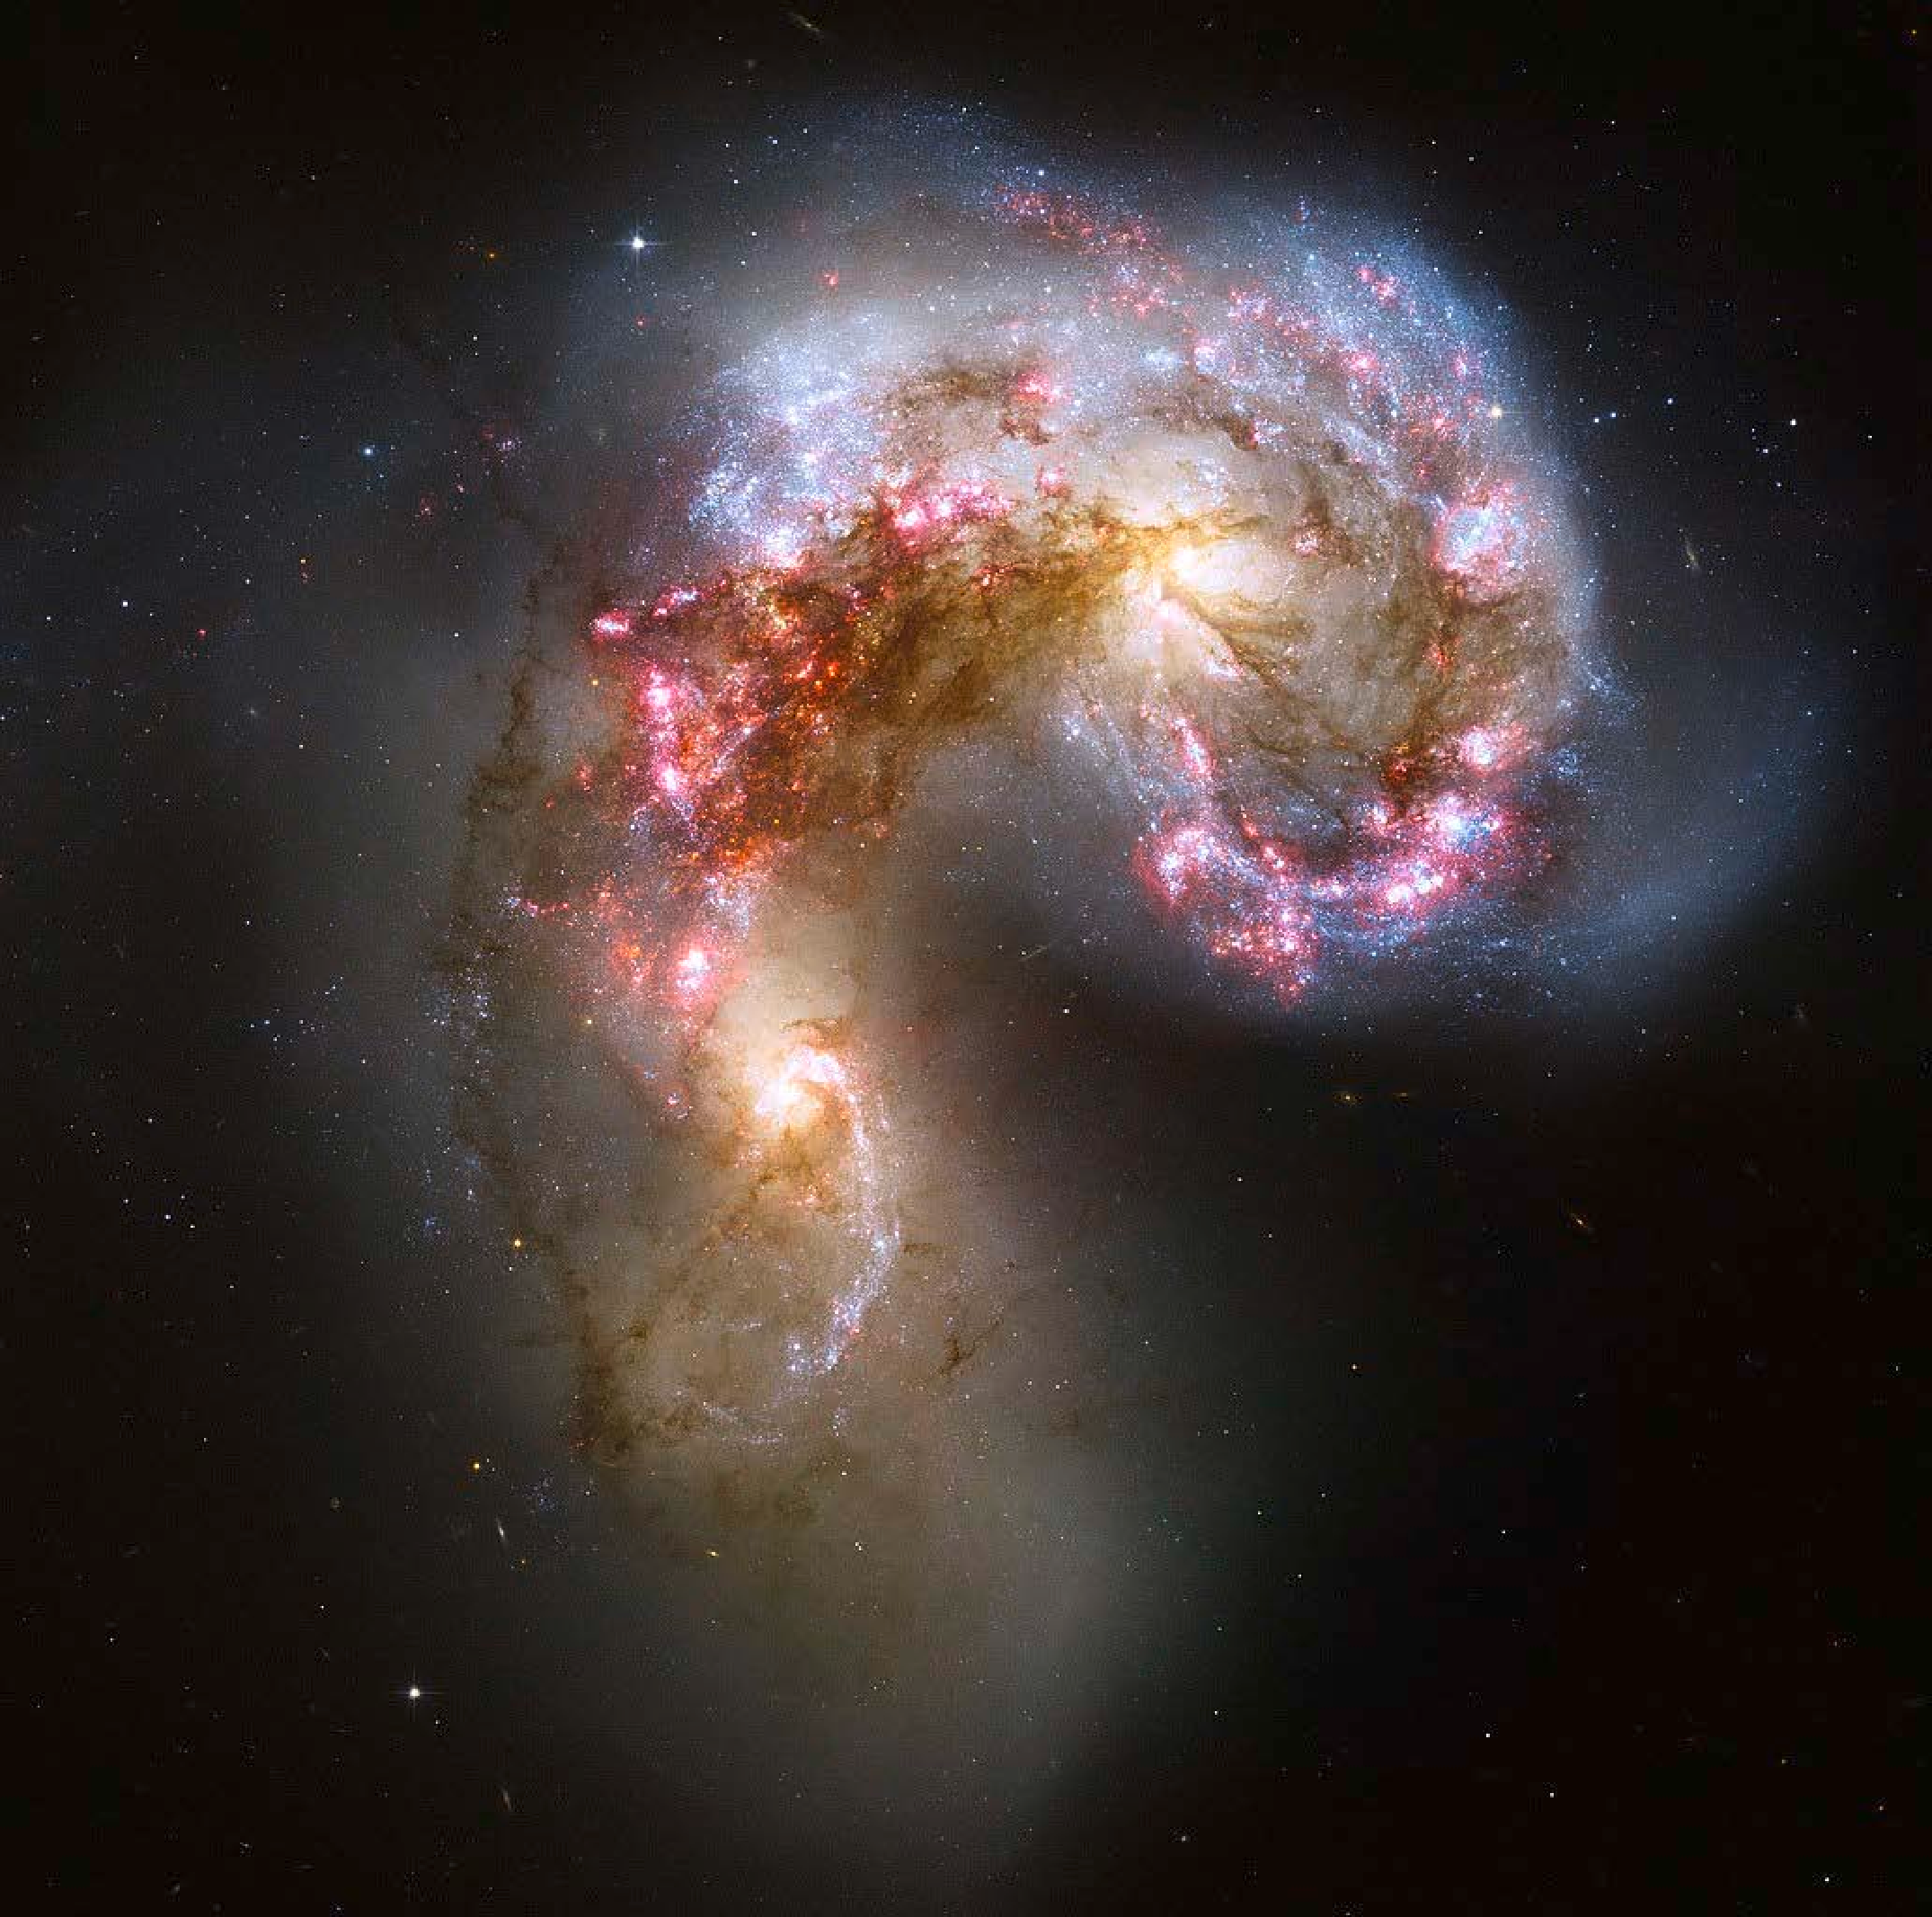
\includegraphics[width=\linewidth]{images/chapters/introduction/sf/Antennae_HST.pdf}
	\caption[Starburst in the Antennae galaxies]{The Antennae galaxies are a proto-typical example of a starburst driven by the tidal interaction and merging of galaxies. The brightest star forming regions host young and forming super star clusters. Source: HST press release \href{https://www.spacetelescope.org/news/heic0615/}{heic0615}.}
	\label{introduction: figure: star formation: Antennae starburst}
\end{figure}

Starbursts can encompass a whole galaxy or just parts thereof, typically, the center. It can be triggered in multiple ways through dynamical forces either by increasing the availability of dense gas or increasing the star formation efficiency \citep[e.g.][]{1991ApJ...370L..65B,1992ARA&A..30..705B}.

The gravitational interaction with other galaxies in major or minor mergers can shock and compress gas which increases the density, allows hot/warm gas to cool and can lead to the formation of dense molecular gas. Tidal forces during the interaction can redistribute angular momentum and drive (molecular) gas to the galaxies' centers where it accumulates to fuel enhanced star formation \citep[e.g.][]{1996ApJ...464..641M}. The Antennae galaxies shown in Figure~\ref{introduction: figure: star formation: Antennae starburst} are an example for a merger or interaction triggered starburst.

Hydrodynamic instabilities in the gas disk of a galaxy can lead to the accumulation of dense gas and therefore enhanced SFR. A typical example are bar instabilities that allow for an efficient transfer of mass into a galaxy's center \citep[e.g.][]{2004ARA&A..42..603K} as is the case in \ngc253 \citep{2000PASJ...52..785S}.
Even if the inflow rate towards the galactic center is not high enough to sustain such a bar-driven starburst, it may be sufficient to ignite periodic short starbursts when the accumulated mass exceeds local limits as is discussed for the Galactic center \citep[e.g.][]{2015MNRAS.453..739K}.


%%%%%%%%%%%%%%%%%%%%%%%%%%%%%%%%%%%%%%%%%%%%%%%%%%%%%%%%%%%%%%%%%%%%%%%%%%%%%%%%%%%%%%%%%%%%%%%%%%%%

\section{Star formation feedback}
\label{introduction: section: star formation: feedback}

\subsection{Mechanisms}
Stars, especially high-mass stars, emit significant amounts of mass, energy and momentum into their surroundings. The combined effect on the ISM is called stellar feedback \citep[e.g.][]{1987ARA&A..25...23S}.
Even before having formed a main sequence star, proto-stellar objects launch gas into their surrounding on stellar ($\LESSSIM$\,pc) scales while accreting from their proto-stellar disk \citep[e.g.][]{1995ApJS..101..117K}.
Once on the stellar main sequence, the fusion processes scale with the stellar mass which causes more massive stars to undergo an increasingly rapid evolution. Hot ($T \GTRSIM 10^4$\,K), young (few Myr) and massive ($M \GTRSIM 3$\,\Msun) O- and B-type stars are violently burning hydrogen and produce intense UV radiation that exerts pressure on the surrounding ISM \citep[e.g.][]{1955ApJ...121....6O,1995ApJ...455..269L}.
Later in the evolution, red giants and supergiants on the asymptotic giant branch (AGB) launch intense, massive stellar winds driven by radiation pressure on the marginally bound outer layers of the stellar atmosphere \citep[e.g.][]{2001A&A...369..574V}. 

Aside from stellar winds, supernovae (SN) are the other important feedback source from evolved stars.
The most massive stars beyond $M \GTR 8$\,\Msun end their life as a core-collapse supernova \citep[SN type II; e.g.][]{1995ApJS..101..181W}. The stellar core eventually reaches temperatures and densities high enough for electrons to combine with protons into neutrons and the electron degeneracy pressure suddenly drops and cannot aid to stabilize the core against gravitational collapse. The implosion of the star then rebounds on the formed neutron core and releases enormous amounts of energy into the stellar envelope that is blown off the star. Typically, only $\sim 20$\% of the pre-SN stellar mass ends up in the remnant meaning that $\sim 80$\% of the mass is ejected, even more when considering the mass loss by stellar winds earlier in the evolution.
Type Ia supernovae occur when an accreting white dwarf crosses the Chandrasekhar mass limit at $M \sim 1.4$\,\Msun and gravitation suddenly dominates over electron degeneracy pressure to trigger collapse and subsequent explosion \citep{1931ApJ....74...81C}.

The kinetic energy ($E \GTRSIM 10^{51}$\,erg) and momentum ($P \GTRSIM 3\times 10^4$\,\Msunyr\,\kms) released by SNe are enormous \citep[e.g.][]{Leitherer:1999jt}.
For a single event, supernovae easily dominate over the other forms of stellar feedback but the sparsity of supernovae ($\sim1$ per 100\,yr for a $SFR \sim 1$\,\Msunyr) limits their impact. In fact, stellar winds and supernovae contribute about equally to the released kinetic energy and momentum of stars \citep[e.g.][]{Leitherer:1999jt}.

For completeness, it needs to be noted that active galactic nuclei (AGN) can also exert feedback on the ISM. Depending on the environment, AGN feedback can add an additional feedback source or completely dominate over stellar feedback.
However, AGN feedback is not relevant for this thesis, so we omit it here.

\subsection{Effect on clouds}
The effect of stellar feedback on the ISM and star formation can be negative (i.e. prevent further star formation), positive (i.e. enhance star formation) or both.
After the first stars have formed in a cloud, their radiation will eventually dissociate, ionize and disperse the remaining (molecular) gas and limit further star formation \citep{2002ApJ...566..302M,2016MNRAS.463.3129G,2018ApJ...853..173K,2018MNRAS.481.2548G}. As such, feedback directly negatively effects the star formation locally by reducing the star formation efficiency of a cloud.
Furthermore, feedback introduces turbulent energy into the ISM that can help to stabilize molecular clouds against gravitational collapse in a state of quasi-static equilibrium \citep{2005ApJ...630..250K,2007ApJ...654..304K,2013ApJ...763...51F}. As such it can provide a preventive feedback loop in the star formation process. The relevant mechanisms are likely proto-stellar outflows on clouds scales \citep[e.g.][]{2010ApJ...709...27W,Krumholz:2012ja,2013A&A...558A..81B} and supernovae on larger up to galactic scales \citep{2016ApJ...822...11P}. It is still debated how much of the released energy and momentum is effectively deposited into the molecular clouds and thus how effective this negative feedback is \citep[e.g.][]{2010ApJ...715.1170A,2015Natur.527...70P,2018ApJ...855...81S}.

On the other hand, feedback creates shocks and (converging) gas flows that can locally enhance the density and enforce self-gravitation of otherwise stable clouds \citep[e.g.][]{1994A&A...290..421W,2012ApJ...744..130K}. Hence, a cloud may obtain more mass from the surrounding ISM that is then converted to stellar mass or it may only be able to become at all self-gravitating by the extra push from feedback. While plausible, the effectiveness of this positive feedback mode is debated \citep[e.g.][]{2015MNRAS.450.1199D,2017MNRAS.464.3536R} and discussed primarily for high redshift AGN feedback \citep[e.g.][]{2015ApJ...799...82C}.
Simulations suggest that both positive and negative feedback may occur side by side in a Galaxy depending on the exact conditions such as gas density and feedback strength \citep[e.g.][]{2017MNRAS.467..512S}


\begin{figure}
	\centering
	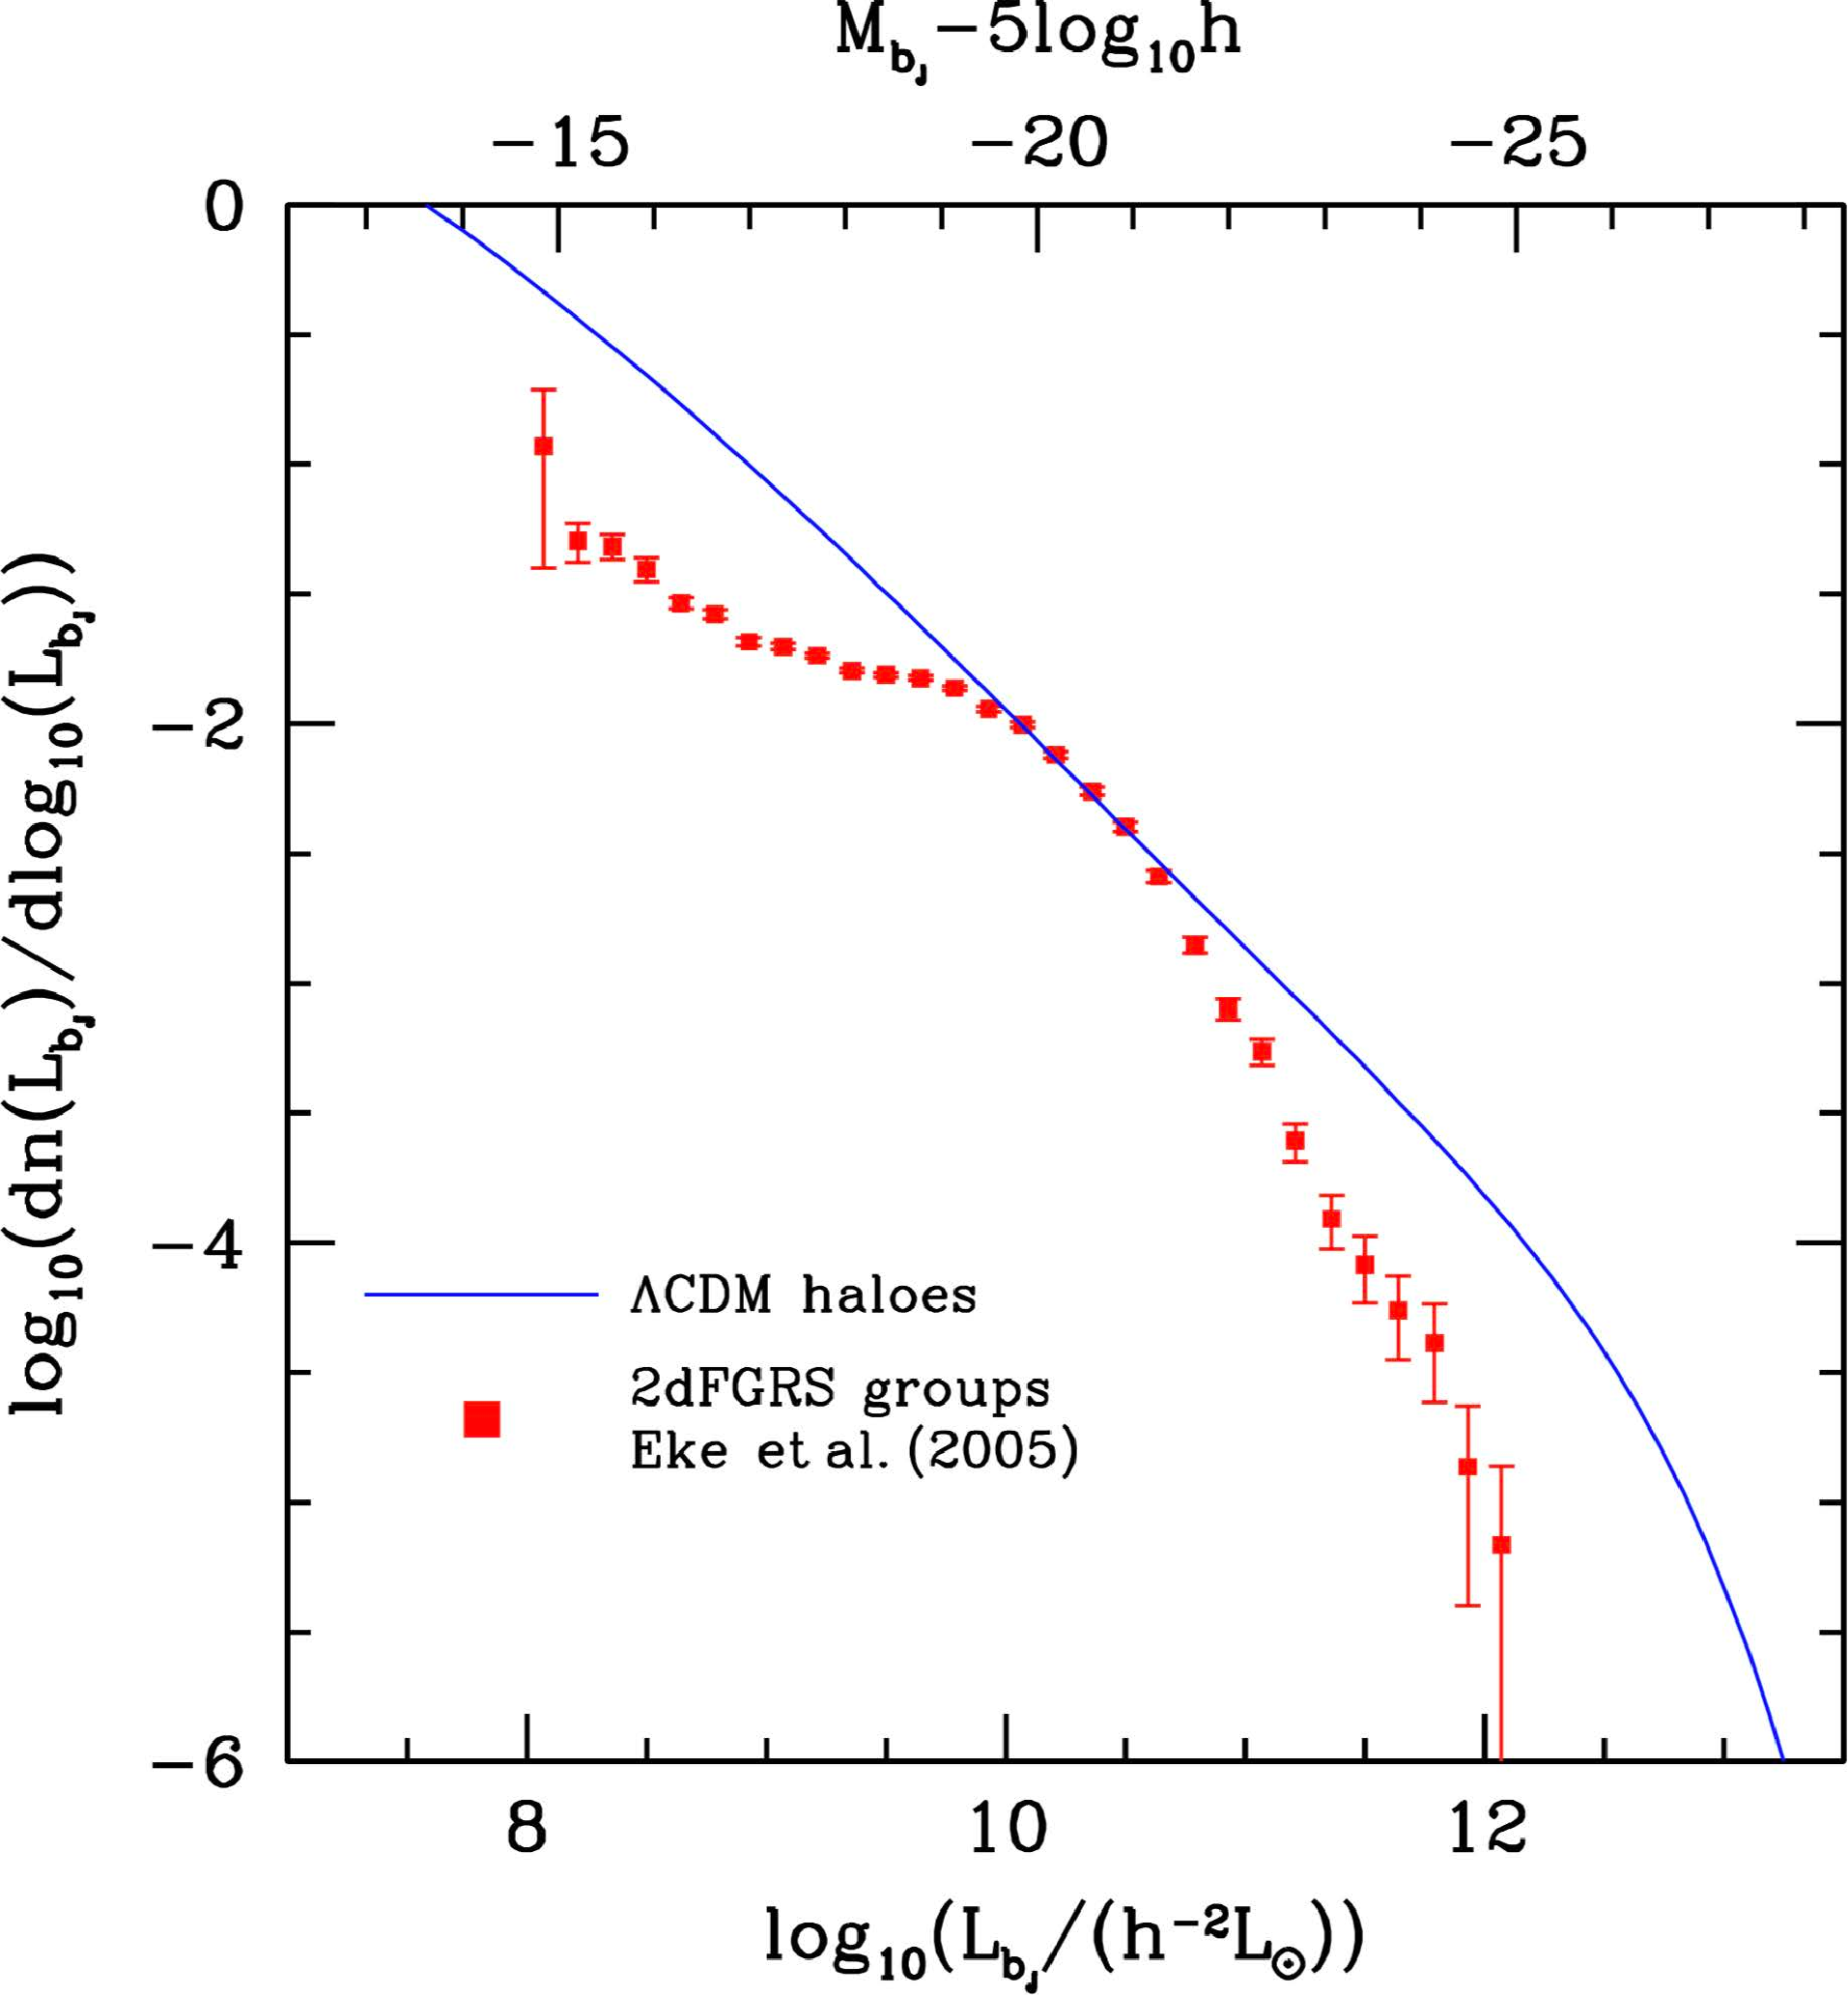
\includegraphics[width=0.55\linewidth]{images/chapters/introduction/sf/luminosity_function.pdf}
	\caption[Galaxy luminosity function compared to the $\Lambda$CDM prediction]{Comparison of the measured galaxy luminosity function (red) to the relation predicted by pure $\Lambda$CDM cosmology (blue). The luminosity function gives the normalized number of galaxies ($n$) as a function of galaxy bolometric luminosity ($L_b$). The mismatch between observations and simple $\Lambda$CDM models at high and low luminosities can be explained by AGN and stellar feedback, respectively. In the lower gravitational potential of dwarf galaxies (low luminosities), supernovae can effectively remove gas by launching outflows and thus suppress the buildup of stellar mass. High-mass galaxies are typically found at the centers of galaxy clusters where frequent interactions funnel gas to the centers resulting in AGN feedback and the shutdown of star formation.
	Figure taken from \citet{2006RPPh...69.3101B}.}
	\label{introduction: figure: star formation: luminosity function}
\end{figure}

\subsection{Effect on galaxies}
Feedback (stellar and AGN) must play a significant role in the formation and evolution of galaxies in the universe. Cosmological simulations not including feedback overpredict the amount of low-mass (low luminosity) but also high-mass (high luminosity) galaxies \citep[e.g.][]{2010gfe..book.....M,2013ApJ...770...57B}. The cosmological standard model $\Lambda$CDM predicts a power law form of the cosmic galaxy luminosity function which is not observed as shown in Figure~\ref{introduction: figure: star formation: luminosity function}. The inclusion of feedback into the models resolve this mismatch. At the low mass end, stellar feedback reduces the number of galaxies by removing gas from the galaxies that is lost for the built-up of stellar mass \citep[e.g.][]{1991ApJ...381...14L,2002MNRAS.330..113K}. At the high mass end, AGNs are increasingly common and thus AGN feedback that inhibits further star formation \citep[e.g.][]{2005MNRAS.361..776S,2006MNRAS.370..645B}.


%%%%%%%%%%%%%%%%%%%%%%%%%%%%%%%%%%%%%%%%%%%%%%%%%%%%%%%%%%%%%%%%%%%%%%%%%%%%%%%%%%%%%%%%%%%%%%%%%%%%

\section{Galactic outflows}
\label{introduction: section: star formation: outflows}

Strong stellar feedback caused by high star formation rate densities can launch outflows of ionized, neutral and molecular gas (Figure~\ref{introduction: figure: star formation: M82 outflow}) that potentially can escape the main body of a galaxy \citep[e.g.][]{1985Natur.317...44C}. Consequently, such outflowing gas removes the potential fuel for future star formation. Therefore, outflows can suppress and quench star formation, as also demonstrated by theoretical predictions and simulations \citep[e.g.][]{1986ApJ...303...39D,2017MNRAS.466.1213K,2018ApJ...857..116M}. Depending on the velocity of the outflow and a galaxy's escape velocity, outflowing gas can be re--accreted at later cosmic times (`galactic fountain' model) or leave the system altogether (`bathtub' model). This process thus has the potential to enrich the galactic disk and circum--galactic medium with metals \citep[e.g.][]{Oppenheimer:2006eq,2010MNRAS.406.2325O,Hopkins:2012ez,Christensen:2018ka}.

\begin{figure}
	\centering
	\includegraphics[width=\linewidth]{images/chapters/introduction/sf/heic0604a.pdf}
	\caption[Outflows in M82]{The large-scale ionized outflow in M82 shows strikingly in this composite image. The optical HST image in the background is overlaid with \Halpha (red) from the Subaru 8.3\,m Telescope. Source: HST press release \href{https://www.spacetelescope.org/news/heic0604/}{heic0604}.}
	\label{introduction: figure: star formation: M82 outflow}
\end{figure}

Galactic outflows are a multi--phase phenomenon and are observed across the electro--magnetic spectrum from X-ray \citep[e.g.][]{2007ApJ...658..258S}, UV \citep[e.g.][]{2005ApJ...619L..99H}, optical like H$\alpha$ \citep[e.g.][]{2009ApJ...696..192W} to IR \citep[e.g.][]{2009ApJ...700L.149V}, cold dust \citep[e.g.][]{2010A&A...518L..66R}, PAH emission \citep[e.g.][]{2006ApJ...642L.127E}, and sub-millimeter to radio including \hi and CO \citep[e.g.][]{2013Natur.499..450B,2015ApJ...814...83L,Lucero:2015if}. Typically, large-scale outflow features at high relative velocity (100s-1000s \kms) are observed in the ionized and neutral gas \citep[e.g.][]{1990ApJS...74..833H,2019MNRAS.486..344R}, whereas molecular outflows often appear as smaller, more compact features \citep[e.g.][]{Strickland:2002kp,Westmoquette:2011bp}. The latter are nonetheless important as they dominate the mass budget \citep{2015ApJ...814...83L}. In some galaxies, the gas phases seem to be stratified with an inner ionized outflow cone, a surrounding neutral shell, and molecular gas situated along the outer edge as is shown in Figure~\ref{introduction: figure: star formation: outflow cone} for \ngc253 \citep[e.g.][]{2015ApJ...801...63M}. Typically, the outflows originate from an extended region, so the apparent outflow cone has its tip cut-off (i.e. a frustum). 

\begin{figure}
	\centering
	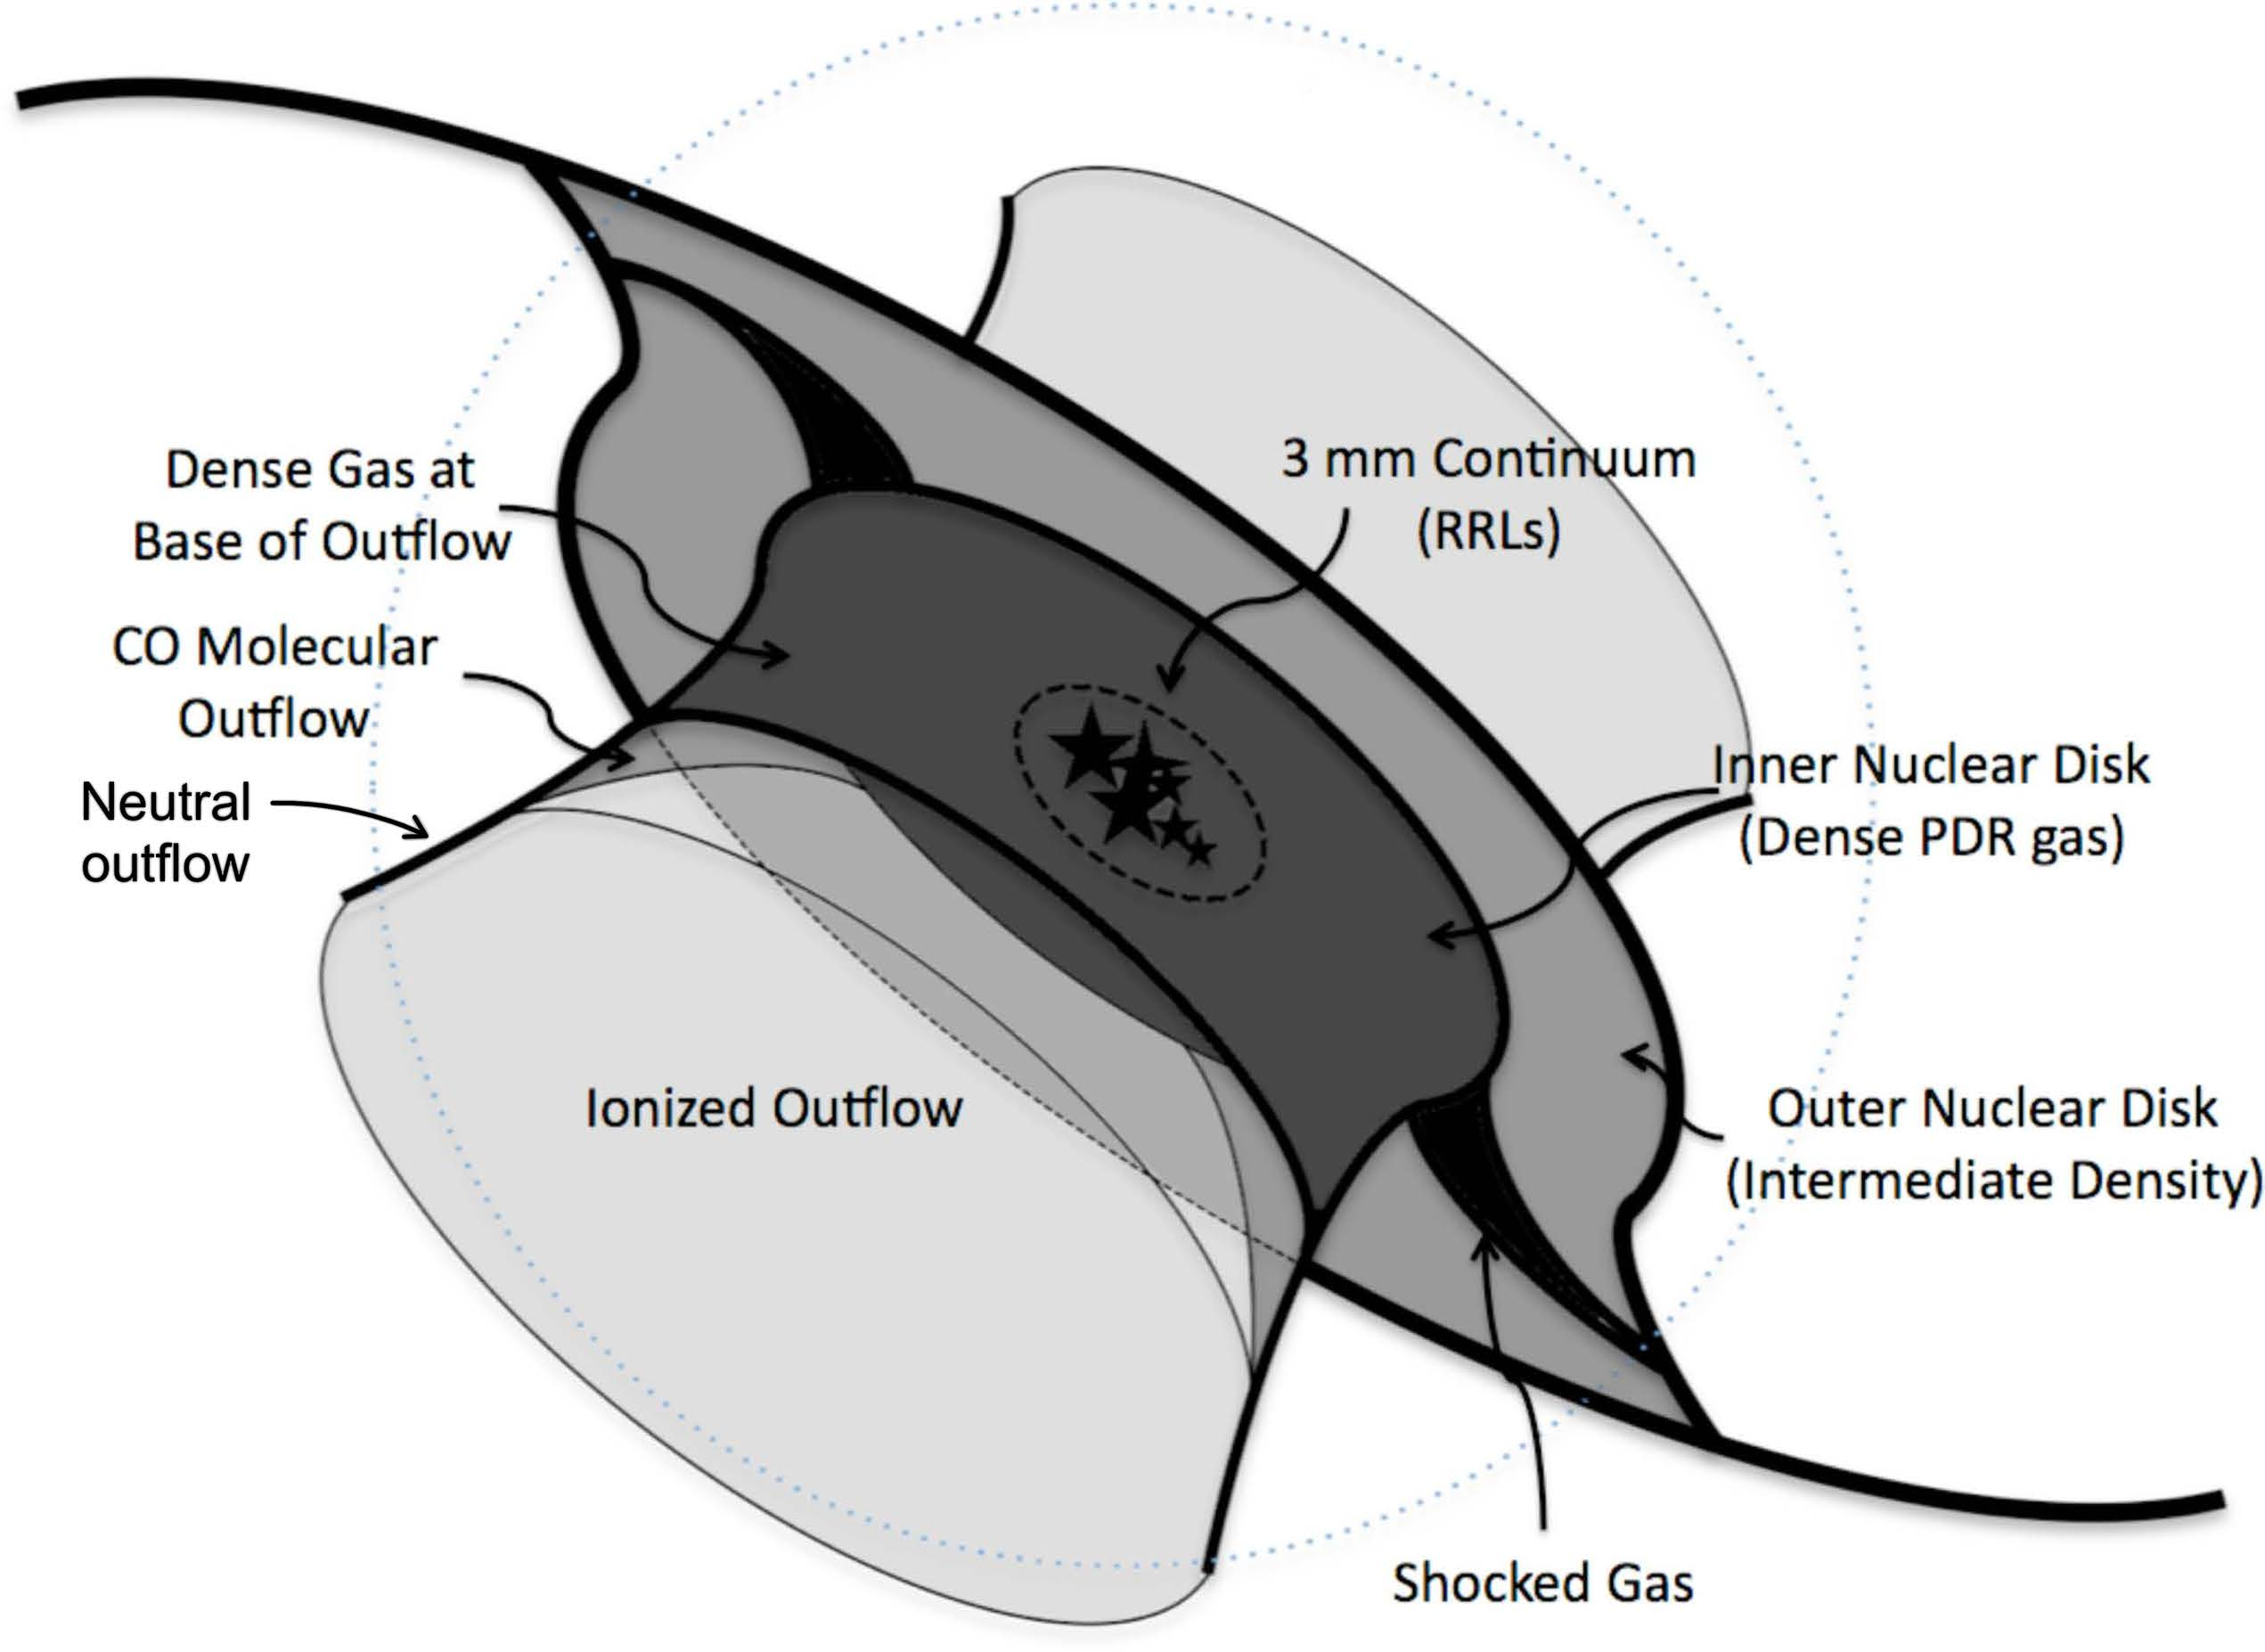
\includegraphics[width=0.7\linewidth]{images/chapters/introduction/sf/outflow_cone.pdf}
	\caption[Schematic of a multi-phase outflow in \ngc253]{Schematic of the multi-phase outflow in \ngc253. The starburst in the center launches a bi-conical stratified outflow. The molecular outflow is thought to be dragged up at the edges of a ionized outflow with a layer of neutral gas in between.
	Figure adapted from \citet{2015ApJ...801...63M}.}
	\label{introduction: figure: star formation: outflow cone}
\end{figure}

Molecular outflows are thus closely intertwined with feedback processes and star formation. The high-resolution structure and kinematic properties of (molecular) outflows have not been studied in detail yet, primarily due to the lack of high resolution and high sensitivity observations. Starburst galaxies are the obvious targets to study star formation-driven outflows due to the high SFR and thus feedback strength in these systems. Consequently, molecular outflows have been studied at tens of parsec scale resolution over the past years in a few nearby starbursts: 
M\,82 \citep{2002ApJ...580L..21W,2015ApJ...814...83L}, NGC\,253 \citep{2013Natur.499..450B,2017ApJ...835..265W,2018ApJ...867..111Z}, NGC\,1808 \citep{2018ApJ...856...97S}, and ESO320-G030 \citep{2016A&A...594A..81P}.


%%%%%%%%%%%%%%%%%%%%%%%%%%%%%%%%%%%%%%%%%%%%%%%%%%%%%%%%%%%%%%%%%%%%%%%%%%%%%%%%%%%%%%%%%%%%%%%%%%%%

\section{Star formation in the cosmological context}
\label{introduction: section: star formation: cosmological context}

\subsection{Cosmic star formation history}

Star formation in galaxies was not steady along the age of the universe but quickly rose in the young universe to then slow down, turn over and decrease \citep[review by][and references therein]{2014ARA&A..52..415M}. The cosmic star formation rate history as shown in Figure~\ref{introduction: figure: star formation: cosmic SFR history} shows this behaviour as a function of redshift and look-back time. At $z\sim2$ when the age of the universe was $\sim 3.5$\,Gyr, the cosmic SFR reached a peak and declined afterwards until today ($z=0$). The shape of the cosmic SFR history is the result of the cosmic expansion starting with the Big Bang and the following coalescence of primordial gas into galaxies that merged into ever larger structures allowing for and triggering star formation. The decline after $z \sim 1.5$ is attributed to a change of accretion mode in galaxies (hot mode vs. cold mode at earlier times) and negative AGN feedback \citep[e.g.][]{2011MNRAS.415.2782V}.

\begin{figure}
	\centering
	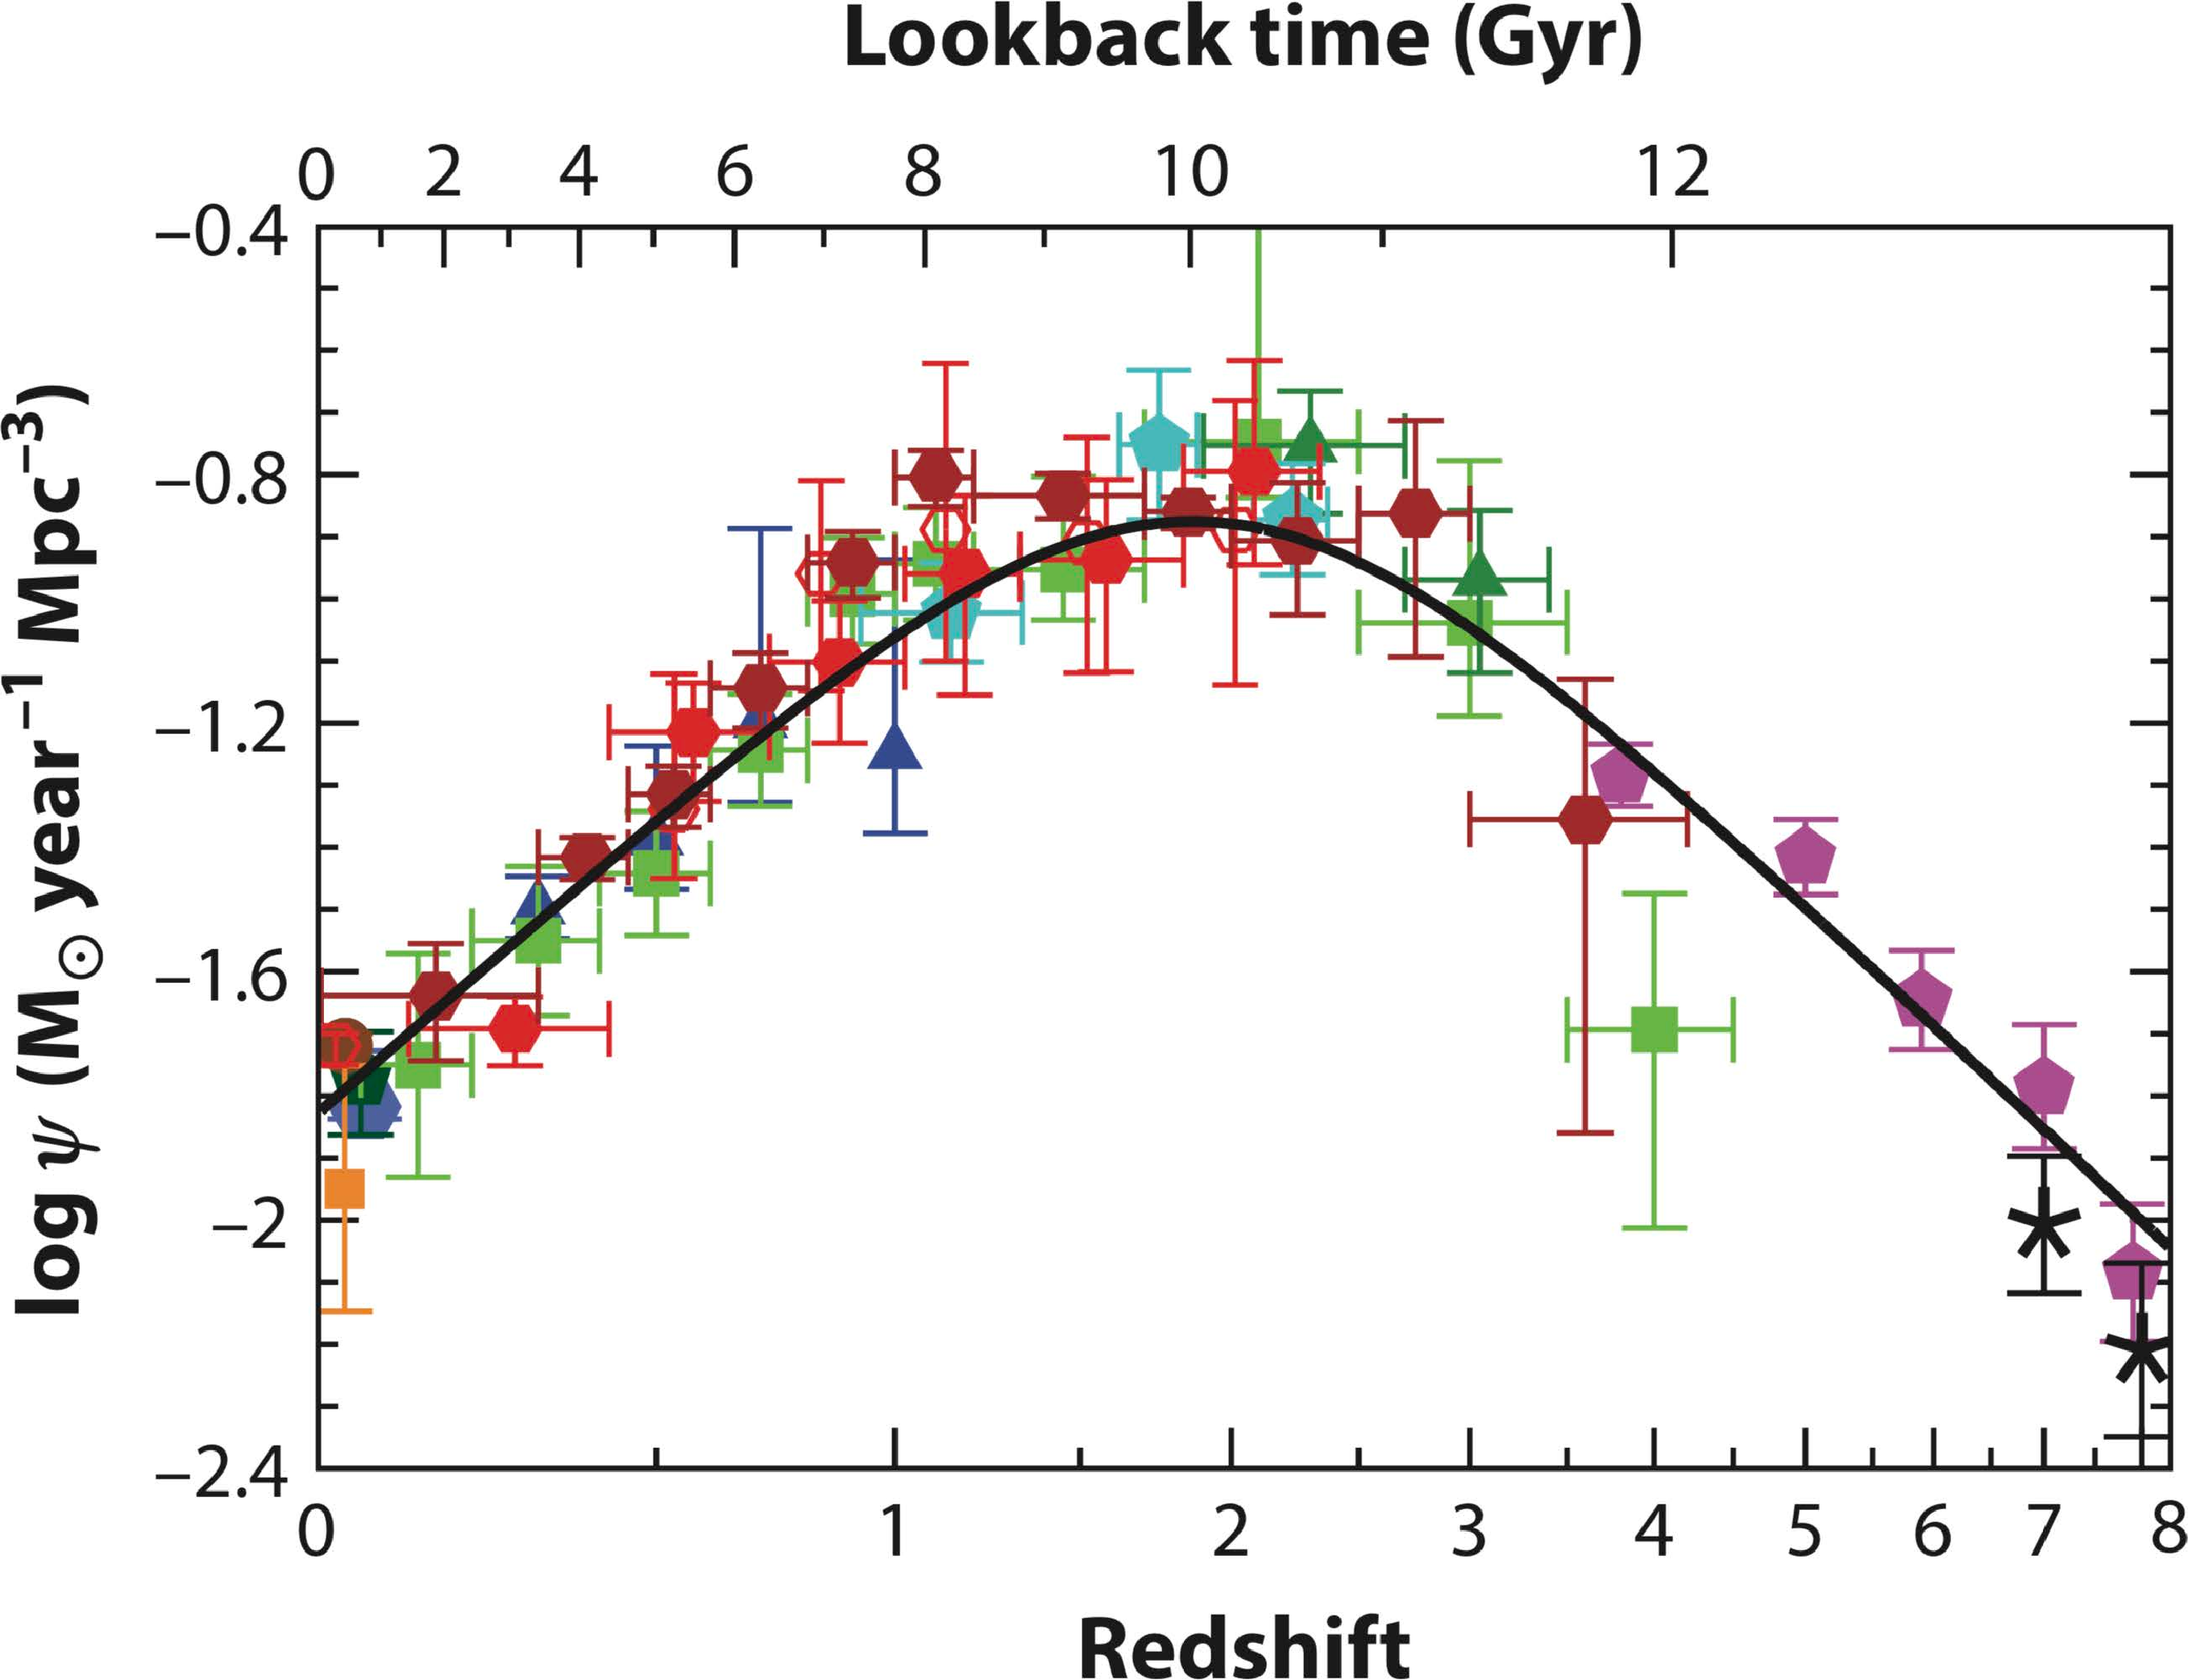
\includegraphics[width=0.6\linewidth]{images/chapters/introduction/sf/csfh.pdf}
	\caption[Cosmic star formation rate history]{Evolution of the cosmic star formation rate density up to redshift $z=8$. In the early universe, star formation quickly became more prevalent and reached a peak at $z\sim2$. At later times, the star formation died down to today's value of $\sim 1$\,\Msunyr per $4^3 = 64$\,Mpc$^3$. At the peak at $z\sim2$, the same volume of the universe had a ten times higher average $SFR \sim 10$\,\Msunyr. Figure adapted from \citet{2014ARA&A..52..415M}.}
	\label{introduction: figure: star formation: cosmic SFR history}
\end{figure}


\subsection{Main sequence evolution}

\begin{figure}
	\centering
	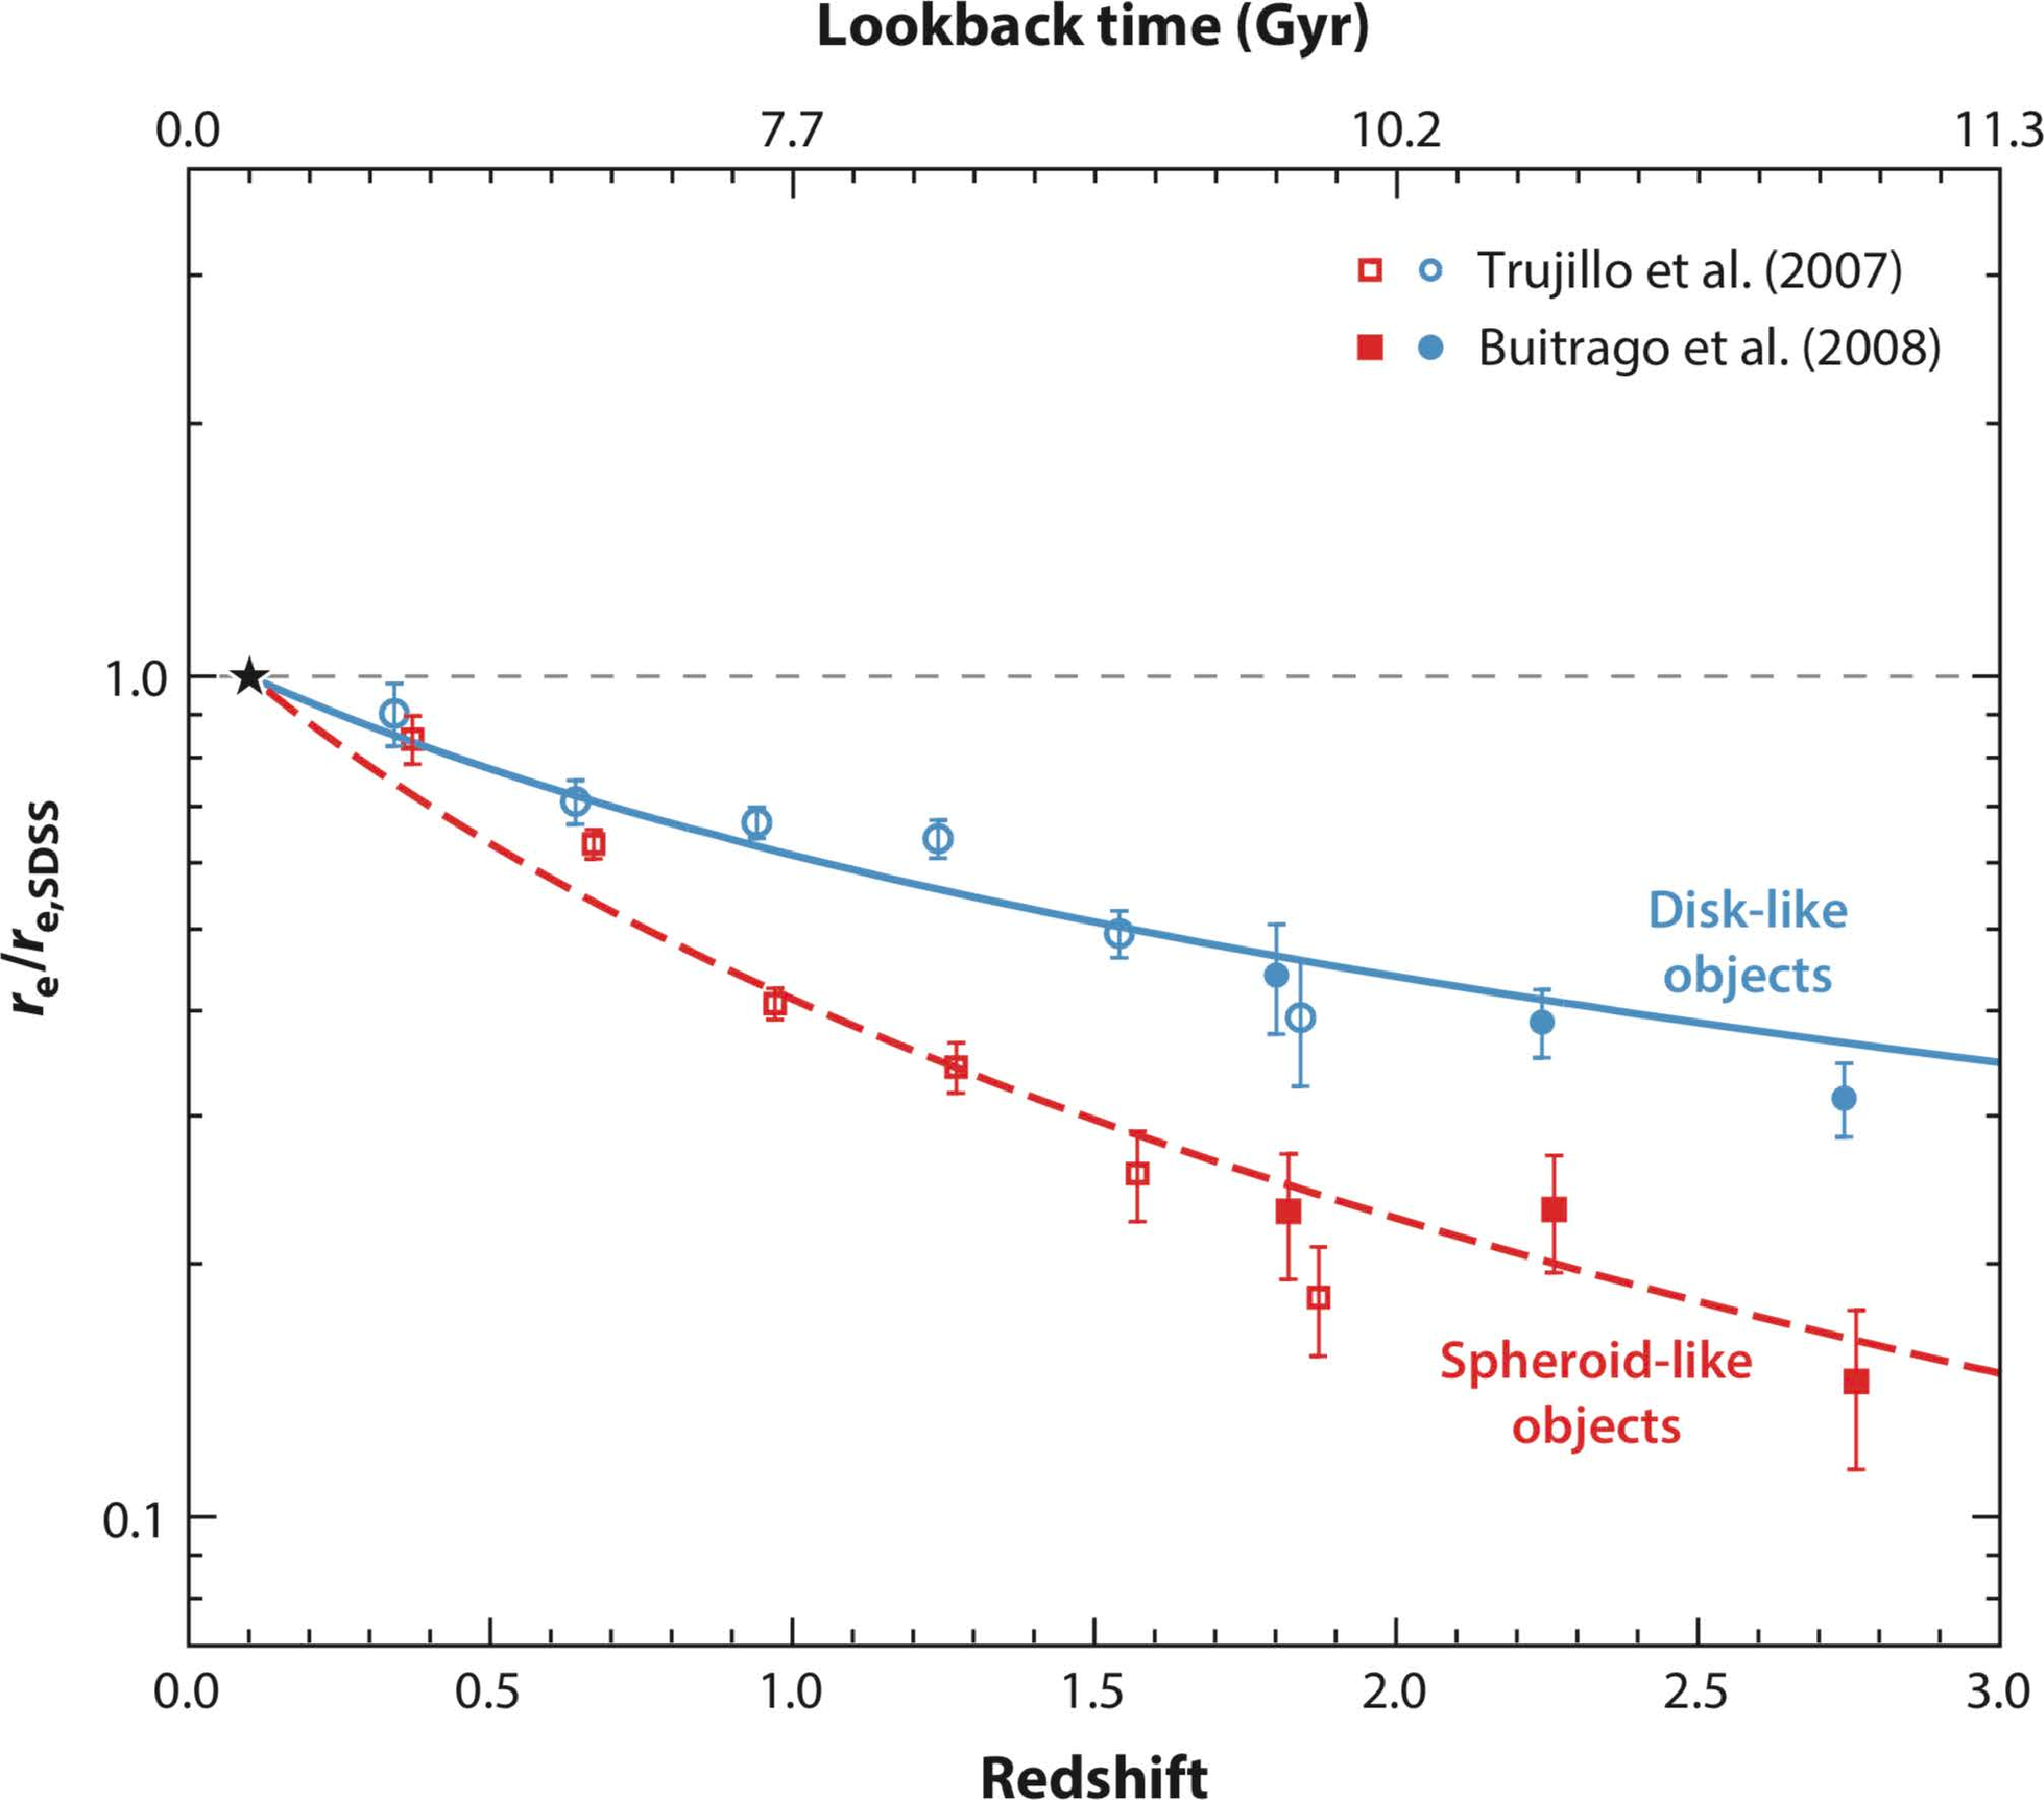
\includegraphics[width=0.6\linewidth]{images/chapters/introduction/sf/size_evolution.pdf}
	\caption[Redshift dependence of galaxy sizes]{Relative average sizes (effective radius $r_\mathrm{e}$) of massive galaxies ($M_* \GTR 10^{11}$\,\Msun) measured by the POWIR and GOODS NICMOS surveys \citep{2007MNRAS.382..109T,2008ApJ...687L..61B}. The reference sizes $r_\mathrm{e,SDSS}$ are derived from $z\sim0$ SDSS galaxies \citep{2003MNRAS.343..978S}. Figure taken from \citet{2014ARA&A..52..291C}.}
	\label{introduction: figure: star formation: galaxy size evolution}
\end{figure}

\begin{figure}
	\centering
	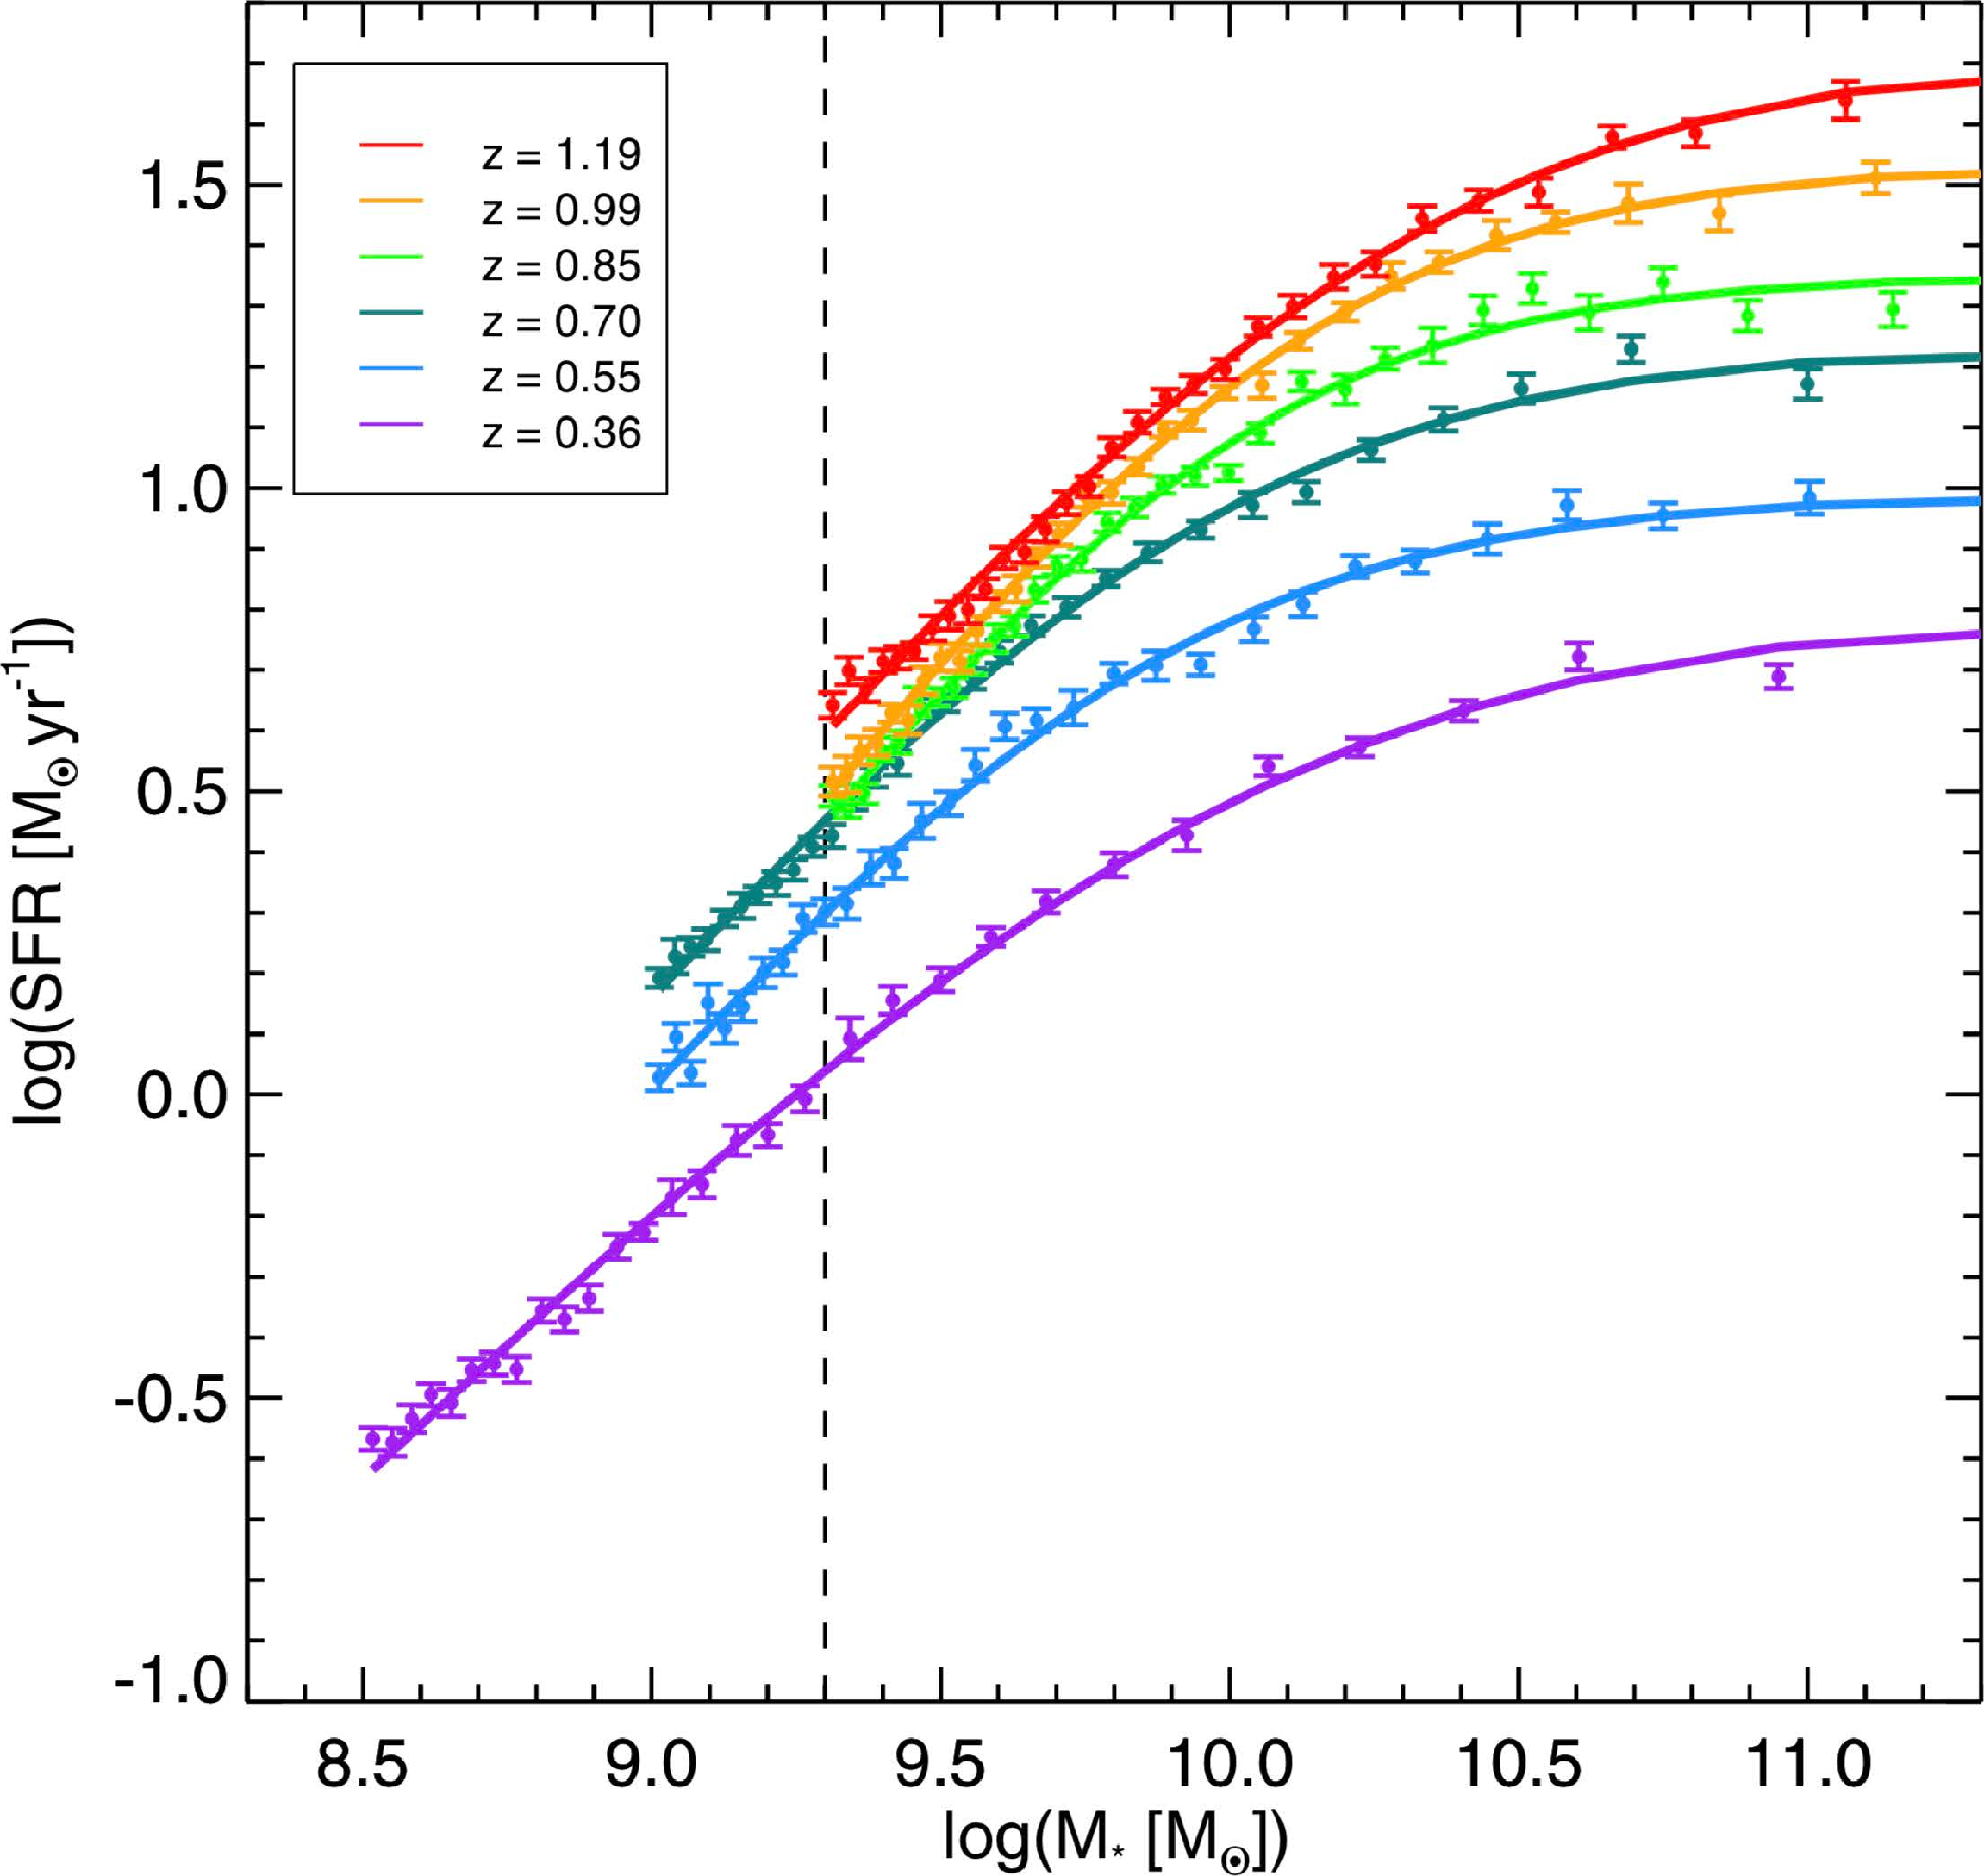
\includegraphics[width=0.6\linewidth]{images/chapters/introduction/sf/ms_shift.pdf}
	\caption[Redshift dependence of the main sequence]{The main sequence of star forming galaxies shifts to higher star formation rate at higher redshift shown here for the range $z =0.36 - 1.19$. In the stellar mass vs. star formation rate plane, a main sequence starforming galaxy at $z \sim 1-2$ would be considered a starburst at $z \sim 0$. Figure taken from \citet{2015ApJ...801...80L}.}
	\label{introduction: figure: star formation: MS shift}
\end{figure}

Similar to the higher SFR density on cosmic scales, the SFR of a typical star forming galaxy also evolves with redshift and is much higher at high-$z$ \citep[e.g.][]{2012ApJ...754L..29W,2014ApJ...795..104W}. Since galaxies grow over time by accretion of gas and galaxy mergers, high-$z$ galaxies are smaller than today's galaxies (Figure~\ref{introduction: figure: star formation: galaxy size evolution}). In combination, a typical high-$z$ star forming galaxy has a greatly enhanced star formation rate surface density $\Sigma_\mathrm{SFR}$ at higher global SFR. The MS (Section~\ref{introduction: section: star formation: main sequence}) thus shifts towards higher SFR with redshift as is shown in Figure~\ref{introduction: figure: star formation: MS shift}. Currently, it is still debated if the shape of the MS also changes with redshift or only shifts up \citep[e.g.][]{2019MNRAS.490.5285P}.

The parameter space above the MS occupied by local ($z \sim 0$) starbursts corresponds to the location of the MS at higher redshift. The correspondence to a particular redshift ($z = 0.5,1,2,...$), of course, depends on the MS offset of the respective starburst. Hence, local starbursts are expected to be analogs or at least proxies to typical star forming galaxies around the peak of the cosmic SFR.


\subsection{Stellar clusters}

As mentioned before in Section~\ref{introduction: section: star formation: SSCs}, SSCs are potential siblings of old globular clusters. To better understand the formation and evolution of globular clusters from local analogs, it must be checked if those local analogs evolve in similar environments and show comparable properties. Observations show that the fraction of stars formed in clusters scales with SFR surface density \citep{2012MNRAS.426.3008K,2016ApJ...827...33J,2018ApJ...864L..17G} and local starbursts show similar $\Sigma_\mathrm{SFR}$ as high-$z$ MS star forming galaxies as explained above. It should therefore be possible to learn more about the formation of the oldest stellar systems by observing SSCs in the nearby universe. Although the general conditions are similar, not much is yet known about the ISM conditions on cluster scales outside the local group. ALMA now offers the resolution and sensitivity to resolve SSCs in e.g. \ngc253 and characterize the physical and chemical properties of the ISM (Chapter~\ref{chapter: SSCs}).


\subsection{The need for local analogs to high-$z$ phenomena}

To resolve the relevant size scales for star formation, ideally pc-scale resolution is required or at least a few tens of pc to resolve GMCs. Achieving such resolutions will be impossible for galaxies at the peak of the cosmic SF history in the short and middle term future. The latest generation of telescopes only achieve resolutions of several hundred pc at $z\GTR1$ --- not nearly enough to resolve SF.
Starbursts as nearby analogs are therefore the most promising and practically the only way to understand how the SF process worked during the most active phase of SF in the universe.

With extremely capable instruments such as ALMA or NOEMA, it is now the time to study the resolved ISM in nearby starbursts to solve how the high-activity mode of SF works and how it affects its host galaxy.


%%%%%%%%%%%%%%%%%%%%%%%%%%%%%%%%%%%%%%%%%%%%%%%%%%%%%%%%%%%%%%%%%%%%%%%%%%%%%%%%%%%%%%%%%%%%%%%%%%%%